\documentclass[times, utf8, zavrsni, numeric]{fer}
\usepackage{booktabs}
\usepackage{multicol}
\usepackage{amsmath}
\usepackage{array}
\usepackage{tabularx}
\usepackage{calc}
\usepackage{subcaption} 
\usepackage{csquotes}
\usepackage{longtable}
\usepackage{changepage}
\usepackage{url}

\newcolumntype {z}[1] {
@ {{\centering \parbox [c]{\tabcolsep}{\rule {0pt}{#1 + 2\tabcolsep}}}}
>{\centering \arraybackslash} m{#1}}
\renewcommand {\tabularxcolumn}[1]{z{#1}}

\newcommand{\STAB}[1]{\begin{tabular}{@{}c@{}}#1\end{tabular}}

\DeclareMathOperator*{\argmax}{arg\,max}

\begin{document}

\thesisnumber{000}

\title{Procjena gustoće mnoštva ljudi utemeljena na matrici pojavnosti lokalnih binarnih uzoraka}

\author{Antonio Kuzminski}

\maketitle

% Ispis stranice s napomenom o umetanju izvornika rada. Uklonite naredbu \izvornik ako želite izbaciti tu stranicu.
\izvornik

\zahvala{}

\tableofcontents

\chapter{Uvod}

U svjetlu problema prouzročenih slabim upravljanjem mnoštva poput
gužvi ili blokada ljudi, postoji povećana potreba za računalnim modelima
koji su sposobni analizirati velika mnoštva ljudi koristeći video prijenos
iz sigurnosnih kamera. Brojenje mnoštva je ključna komponenta takvih 
automatiziranih sustava za analizu gustoće mnoštva. Sustav uključuje 
procjenu broja ljudi u mnoštvu kao i distribuciju gustoće mnoštva
dotičnog mjesta. Identifikaicija regija s gustoćom mnoštva većom
od neke sigurne granice može pomoći kod izdavanja upozorenja i spriječiti
potencijalne gužve. Procjena broja grupacija mnoštva može doprinijeti
do bolje raspodjele ljudi, resursa i logistike kod organizacije događaja
kojem prisupa veći broj ljudi ili kontroliranje već postojećih, npr. 
utakmica, prosvjedi ili bilo kakva slična okupljanja.

\bigbreak

Mnoštva mogu biti vrlo različita, npr. po svojoj prostornoj razdiobi, smjeru kretanja ili međusobnim djelovanjem. Predloženo 
je puno metoda koje se zasnivaju na značajkama teksture za rješavanje ovog
problema. Većina postojećih metoda procjenjuje gustoću mnoštva na razini
cijele slike pritom ignorirajući lokalna područja. U ovom radu predlaže se
metoda bazirana na matrici pojavnosti lokalnih binarnih značajki
(engl. \textit{Local binary pattern co-occurrence matrix - LBPCM}).

\bigbreak

Matrica se konstruira na svakom oknu podslike te se iz te matrice izračunaju 
Haralickove značajke koje se zatim dodaju u vektor značajki. Iako je 
gustoća mnoštva definirana kao broj ljudi po jedinici površine, 
brojanje ljudi nije uvijek potrebno za analizu gustoće. Polus i 
drugi \citep{polus} prvi su predstavili tok mnoštva koji je uvelike prihvaćen. 
Prema njima gustoća mnoštva može se svrstati u četiri razreda: 
slobodan tok, ograničen tok, gusti tok i zakrčen tok. 
LBPCM opisuje statistička svojstva, ali isto tako i prostornu 
informaciju pritom iskorištavajući puni potencijal LBP-a za 
lokalne značajke teksture. Dodatno, konstruiramo LBPCM na sivim i 
gradijentnim slikama u svrhu poboljšanja točnosti klasifikacije.


\chapter{Teorijske osnove}
U ovom poglavlju objašnjavaju se detaljnije termini i metodologije korištene u radu.

\subsection{LBP (engl. \textit{Local binary pattern}) - lokalna binarna značajka}

LBP se razvio kao poseban slučaj jedinice teksture (\textit{engl. Texture unit})
koje je prvi put predstavljena u radu \citep{dong}.
Jedinica teksture se definira na sljedeći način. 

\bigbreak

U kvadratnoj rasterskoj digitalnoj slici svaki piksel okružen je s
osam susjednih piksela (osim krajnjih piksela na rubu slike). 
Lokalna informacija teksture izvlači se iz susjedstva 3x3 koje 
predstavlja najmanju potpunu jedinicu (u smislu postojanja osam 
smjerova oko piksela). Obzirom na 3x3 susjedstvo koje će biti 
označeno skupom od devet elemenata \(V = \left\{V_0, V_1,..., V_8\right\}\),
gdje \(V_0\) predstavlja intenzite srednjeg piksela, a 
\(\left\{V_0, V_1,..., V_8\right\}\) predstavlja entiteta susjednih piksela.
Jedinica teksture je skup od osam elemenata TU = \(\left\{E_1, V_2,..., E_8\right\}\),
gdje su \(E_i = (0,1\; ili \;2)\) i određuje se formulom

\[
E_i = \left\{
\begin{matrix}
0, \; ako \; je \; V_i \le V_0 \\
1, \; ako \; je \; V_i = V_0 \\
2, \; ako \; je \; V_i \ge V_0 \\
\end{matrix}
\right.
\]

za sve \(i=1,2,...,8\). Kako svaki element TU ima 3 mogućnosti, ukupno
postoji \(3^8 = 6561\) jedinica teksture. Broj \(N_{TU}\) predstavlja 
pojedinu jedinicu teksture, a dobiva se na sljedeći način:

\[
N_{TU} = \sum_{i=0}^{8} E_i \cdot 3^{i-1}
\]

\newpage

Moguće je elemente poredati na različite načine, ali se uzima 
način prikazan na slici 2.1. Prvi element je element \(a\), zatim \(b\) i 
tako sve do \(h\).  

\bigbreak

\begin{minipage}{\linewidth}
\centering
\begin{tabularx}{0.25\textwidth}{| X | X | X |}
\hline
a & b & c \\ 
\hline
h &  & d  \\ 
\hline
g & f & e  \\
\hline
\end{tabularx}
\captionof{figure}{Prikaz poretka jedinica teksture u susjedstvu srednjeg piksela.}
\end{minipage}

\vspace{0.7cm}

\underline{\textbf{Primjer} - Dobivanje teksturne jedinice}

\bigbreak

\begin{minipage}{\linewidth}
\centering
\begin{tabularx}{0.25\textwidth}{| X | X | X |}
\hline
62 & 20 & 41 \\ 
\hline
79 & 40 & 30 \\ 
\hline
130 & 40 & 10 \\
\hline
\end{tabularx}
\captionof{figure}{Susjedstvo V = \{40, 62, 20, 41, 30, 10, 40, 130, 79\}}
\end{minipage}

\bigbreak

\begin{minipage}{\linewidth}
\centering
\begin{tabularx}{0.25\textwidth}{| X | X | X |}
\hline
2 & 0 & 2 \\ 
\hline
2 &  & 0 \\ 
\hline
2 & 1 & 0 \\
\hline
\end{tabularx}
\captionof{figure}{Jedinica teksture TU = \{2, 0, 2, 0, 0, 1, 2, 2\}}
\end{minipage}


\begin{center}
\(TU = 2 \cdot 3^0 + 2 \cdot 3^2 + 3^5 + 2 \cdot 3^6 + 2 \cdot 3^7 + 2  = 6095\)
\end{center}

\medskip

Nakon definicije jedinice teksture, lako je objasniti lokalnu binarnu značajku. 
LBP se izračunava na potpuno jednak način osim što postoje samo dvije vrijednosti 
(0 i 1) umjesto 3. Ovakav način predložen je od \citep{ojala}. Ovaj 
pristup je pogodniji jer postoji ukupno \(2^8\)  = 256 različitih kombinacija LPB-a, 
odnosno toliko koliko ima i razina svjetline pa su zbog toga slike u sivim 
razinama prigodne.


\begin{multicols}{2}

\begin{minipage}{\linewidth}
\centering
\begin{tabularx}{0.4\textwidth}{| X | X | X |}
\hline
1 & 1 & 1 \\ 
\hline
0 &  & 1 \\ 
\hline
0 & 0 & 1 \\
\hline
\end{tabularx}
\captionof{figure}{Susjedstvo nakon usporedbe s centralnim pikselom}
\end{minipage}

\begin{minipage}{\linewidth}
\centering
\begin{tabularx}{0.4\textwidth}{| X | X | X |}
\hline
71 & 171 & 190 \\ 
\hline
5 & 55 & 78 \\ 
\hline
24 & 12 & 78 \\
\hline
\end{tabularx}
\captionof{figure}{Susjedstvo V = \{55, 71, 171, 190, 78, 78, 12, 24, 5\}}
\end{minipage}

\end{multicols}

\[LBP = 2^0 + 2^1 + 2^2 + 2^3 + 2^4 = 31\]

\bigbreak

Slika 2.5 prikazuje jednu sliku sivih razina.
U prethodnim primjerima razmatrano je susjedstvo udaljeno samo za 
jedan piksel, međutim, to ne mora uvijek biti tako. Moguće je 
definirati susjedstvo kao kvadratno susjedstvo radijusa, npr. 3, što za sobom 
povlači veći broj piksela koji sudjeluju u nastajanju LBP-a. 

\bigbreak

Primjer slike dimenzija 64x64 i primijenjenog LBP operatora na tu 
sliku s radijusom redom 1, 2 i 3.

\begin{figure}[ht]
\begin{subfigure}[b]{0.24\linewidth}
\centering
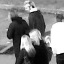
\includegraphics{img/1.jpg}
\end{subfigure}
\begin{subfigure}[b]{0.24\linewidth}
\centering

\includegraphics{img/2.jpg}
\end{subfigure}
\begin{subfigure}[b]{0.24\linewidth}
\centering

\includegraphics{img/3.jpg}
\end{subfigure}
\begin{subfigure}[b]{0.24\linewidth}
\centering

\includegraphics{img/4.jpg}
\end{subfigure}

\caption{Primjer dobivenih LBP slika iz izvorne slike uz različite radijuse oko centralnog piksela}
\end{figure}

Kao dodatno proširenje na osnovni operator LBP je takozvani jednolični uzorak 
(engl. \textit{uniform pattern}) koji može biti korišten za smanjenje dimenzija
vektora značajki, ali i kao jednostavni deskriptor otporan na rotaciju slike 
\citep{barkan}. Ideja je motivirana činjenicom da se neki 
binarni uzorci pojavljuju više od nekih drugih u slikama s teksturom. 
LBP se naziva jednoličnim ako ima najviše dvije 0-1 ili 1-0 tranzicije.
 Npr. 00010000 ima dvije tranzicije, ali 01010100 ima šest tranzicija 
 i on nije jednoličan. U izračunima LBP histograma, svaki uzorak ima 
 svoju grupu (poziciju), a svi koji nisu jednolični uzorci se 
 svrstavaju u zajedničku grupu. Koristeći jednolične uzorke,
  dimenzionalnost vektora značajki možemo smanjiti sa 256 na 59 
  (toliko ima jednoličnih uzoraka ako koristimo radijus jedan piksel).

\newpage

\subsection{Matrica pojavnosti sivih razina}

Matrica iz naslova predložena je od strane Haralicka i dr. \citep{haralick}, 
a Marana \citep{marana} je koristi za procjenu gustoće mnoštva.
Tipično se matrica izračunava nad crno bijelim slikama, odnosno slikama sivih razina,  pa je poznatija
pod imenom matrica pojavnosti sivih razina (engl. \textit{Gray level co-occurence matrix - GLCM}).

\bigbreak

GLCM je statistička metoda procjene združenih uvjetnih vjerojatnosnih funkcija
gustoće \(f(i,j,d,\theta)\). Svaka \(f(i,j,d,\theta)\) predstavlja vjerojatnost 
da se par sivih razina \((i,j)\) javlja na udaljenosti \(d\) u smjeru \(\theta\)
na slici. Korištenje izvorne matrice u učenju različitih sustava klasifikacije 
je nepraktično jer sadrži veliku količinu informacije pa se zbog toga koriste
Haralickove značajke koje su prikazane u dodatku A. Dimenzionalnost GLCM
je uvjetovana brojem sivih razina slike nad kojom se izračunava matrica.

\bigbreak

Primjer računanja matrice pojavnosti sivih razinai za \(d=0, \theta=0\). Slika 
sa sivim razinama koja služi za izračunavanje funkcije \(f(i,j,1,0)\) nalazi 
se na slici 2.7.

\bigbreak
\bigbreak

\begin{minipage}{\linewidth}
\centering
\begin{tabularx}{0.3\textwidth}{| X | X | X | X |}
\hline
0 & 0 & 1 & 1 \\ 
\hline
0 & 0 & 1 & 1 \\ 
\hline
0 & 2 & 2 & 2 \\
\hline
2 & 2 & 3 & 4 \\
\hline
\end{tabularx}
\captionof{figure}{Primjer crno bijele slike}
\end{minipage}

\bigbreak

Postupak dobivanja elemenata matrice \(f(i,j,1,0)\) opisan je u sljedećim koracima i zatim
je prikazan izgled same matrice te izgled kada je provedena normalizacija matrice. 
Uzmimo da indeksi počinju od 0 i kao primjer
element \((0,0)\) koji predstavlja sva pojavljivanja dviju nula na udaljenosti 1
u smjeru od 0 stupnjeva, odnosno udesno. Iz slike je vidljivo da postoje takva
dva mjesta: prvi i drugi redak. Stoga se u matricu \(f(i,j,1,0)\) na mjestu
s indeksom \((0,0)\) upisuje broj 2. 

\bigbreak

Kao sljedeći element uzmimo \((2,3)\).
Potrebno je pronaći gdje se u izvornoj slici nalaze sive razine intenziteta
2 i 3 jedna kraj druge na udaljenosti 1 udesno. Iz slike je vidljivo da 
jedino mjesto pojave takvih razina u zdanjem retku, stoga u \(f(i,j,1,0)\)
na mjestu s indeksima \(2,3\) upisujemo 1. 

\bigbreak

Daljnjim nastavkom istog postupka
dolazi se do krajnjeg oblika matrice \(f(i,j,1,0)\) koja izgleda ovako

\bigbreak

\begin{figure}[ht]
	\begin{subfigure}[b]{0.49\linewidth}
		\begin{minipage}[b]{\textwidth}
			\centering
			\small
			\(
			\begin{bmatrix}
			2&2&1&0\\
			0&2&0&0\\
			0&0&3&1\\
			0&0&0&1\\
			\end{bmatrix}
			\)
			\caption{prije normalizacije}\label{first}
		\end{minipage}\hfill
	\end{subfigure}
	\begin{subfigure}[b]{0.49\linewidth}
		\begin{minipage}[b]{\textwidth}
			\centering
			\small
			\(
			\begin{bmatrix}
			0.167&0.167&0.083&0\\
			0&0.167&0&0\\
			0&0&0.25&0.083\\
			0&0&0&0.083\\
			\end{bmatrix}
			\)
			\caption{nakon normalizacije)}\label{first}
		\end{minipage}\hfill
	\end{subfigure}
\caption{Prikaz GLCM prije i nakon normalizacije}
\end{figure}

\bigbreak

Prikazana GLCM je oblika 4x4 jer sive razine izvorne slike mogu poprimiti
4 različite vrijednosti. U radu se koriste slike zapisane u 8-bitnom formatu
što znači da se veličina matrice povećava na \(256,256\) jer svaki piksel može
poprimiti jednu od 256 različitih vrijednosti. Zbog veličine matrice mnoge
kombinacije razina piksela se često ne pojavljuju u izvornim slikama što
dovodi do toga da su matrice dosta prazne, odnosno puno indeksa imaju popunjene 
nulama.

\bigbreak

\underline{\textbf{Primjer} - Dobivanje vrijednosti Haralickove značajke - energija.}

\bigbreak

Uzmimo izvornu sliku. Energija se računa prema
\[
f_1 = \sum_{i}\sum_{j}p(i,j)^2
\]

gdje \(p(i,j)\) označava vrijednost GLCM za udaljenost 1 i kut od 0 stupnjeva.

\[
f_1 = 3 \cdot 0.167^2 + 3 \cdot 0.083^2 + 0.25^2 = 0.166834
\]

U ovom radu se koristi matrica naziva LBPCM (engl. \textit{Local binary pattern co-occurence matrix})
koja je u suštini GLCM samo što se izračnavanje vriijednosti matrice 
radi nad slikom sivih razina nad kojom je primijenjen operator LBP.

\newpage

\subsection{Klasifikator \textit{k} najbližih susjeda - \textit{k}-NN}

Ovaj klasifikator je jednostavan nadziran (engl. \textit{supervised})
algoritam strojnog učenja koji može biti korišten za klasifikaciju
i regresije. Problemi klasifikacije imaju kao izlaz diskretne vrijednosti
dok s druge strane problemi regresije na izlazu poprimaju realne vrijednosti.
\textit{k}-NN algoritam pretpostavlja da se slične stvari nalaze 
jedne blizu drugih.

\bigbreak

Nadzirani algoritmi strojnog učenja oslanjaju se na označene početne uzorke
podataka kako bi dobili (naučili) funkciju koja daje prikladnu izlaznu vrijednost
kada joj se preda neki, još do sada neviđeni uzorak. 

\bigbreak

Slovo \textit{k} u nazivu \textit{k}-NN predstavlja broj susjeda koji sudjeluju
u \enquote{glasanju}. To glasanje predstavlja dodjeljivanje labele od strane \textit{k}
najbližih susjeda. Ukiliko je \(k=1\), labelu određuje samo najbliži susjed,
ako je \(k=3\), razred s više glasova pobjeđuje te se kao labela novome, dosad
nevđenome uzorku, dodjeljuje baš taj razred. Za broj susjeda se odabire pozitivan
broj koji je tipično malen. Kako bi odabrali dobru vrijednost broja \textit{k} poželjno
je algoritam pokrenuti nekoliko puta. 

\begin{multicols}{2}

Smanjenjem broja \textit{k} odluke postaju
sve nestablinije, npr. ako postoji jedan primjer nekog drugog 
razreda (koji previše odskače od vrijednosti svoga razreda) u blizini suprotnog razreda, 
može doći do krive klasifikacije što bi se inače izbjeglo povećanjem broja \textit{k}. 
Crna točka iz slike 2.9 prikazuje još neklasificiran uzorak. 

\begin{minipage}{\linewidth}
\vspace{10pt}
\centering
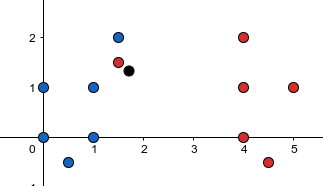
\includegraphics[width=0.8\linewidth]{img/krivo.png}
\captionof{figure}{Prikaz dva razreda s jednim nestandardnim uzorkom (koji previše odskače od prosjeka uzoraka svojeg razreda)}
\end{minipage}

\end{multicols}

\bigbreak
Ukoliko bi kao konstantu \textit{k} izabrali 1, novi uzorak bi se klasificirao 
u crveni razred, a iz slike je jasno vidljivo da to nije poželjno. Točnost 
klasifikacije nije samo uvjetovana izborom konstante \textit{k}. Naime, 
ako su grupe pojedinih razreda raštrkane, odnosno njihov oblik je nepravilan,
točnost klasifikacije se narušava. Uspješnost algoritma može biti 
značajno degradirana korištenjem nekih značajki u vektorima koje ne 
doprinose međusobnoj diskriminaciji pojedinih vektora ili su skale pojedinih 
komponenti vektora neprilagođene njihovoj značajnosti pa je njihov ukupan doprinos prevelik. 

\newpage

\underline{\textbf{Primjer} - Klasifikacija \textit{k}-NN klasifikatorom. }

\bigbreak

Raspored uzoraka prikazan je na slici 2.10. Postoje 2 razreda - crveni i plavi. 
Uzorak koji se pokušava klasificirati označen je crnom bojom. 

\begin{minipage}{\linewidth}
\vspace{10pt}
\centering
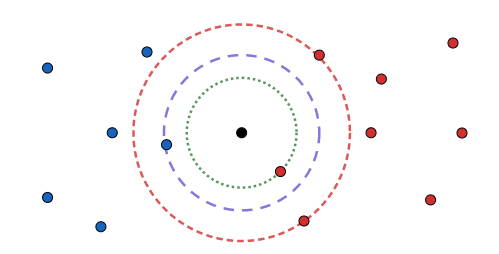
\includegraphics[width=0.8\linewidth]{img/klas.png}
\captionof{figure}{Prikaz uzoraka dva razreda i novog uzorka za klasifikaciju}
\end{minipage}

\bigbreak

Odabirom konstante \textit{k} utječemo na krajnju dodjelu labele.

\begin{itemize}
	\item \(k=1\) - Slučaj je prikazan crtkanom kružnicom zelene boje (kružnica najmanjeg 
	radijusa). Pripadnost se određuje na temelju najblžeg susjeda pa labela
	novog uzorka postaje crveni razred.
	\item \(k=2\) - Najbliža dva susjeda. Slučaj je prikazan plavom crtkanom kružnicom.
	Ovakva situacija nije poželjna jer se unutar granica nalazi jednak 
	broj pripadnika svakog od razreda. Kako bi razriješili situaciju mogli bi uzeti
	kao dodatnu mjeru udaljenost svakog od uzoraka unutar kružnice do novog uzorka te
	pridodijeliti labelu bližeg. Kako bi izbjegli ovakve situacije dobra je praksa 
	uzimati neparne vrijednosti konstante \textit{k}.
	\item \(k=3\) - Situacija označena kružnicom najvećeg radijusa. Vidljivo
	je da su većinski pripadnici crvenog razreda unutar granica pa se
	novome uzorku dodjeljuje labela crvenog razreda.
\end{itemize}

\newpage

\subsection{Stroj s potpornim vektorima (engl. \textit{Support vector machine - SVM}}

Ovaj klasifikator pripada vrsti linearnih klasifikatora što znači da 
ako postoji neki skup vektora X u kojem svaki od vektora \(x_i, i = 0, 1, ..., N\), 
pripada jednom od razreda \(\omega_1\) ili \(\omega_2\) te su ti razredi odvojivi hiperravninom 
u prostoru dimenzionalnosti \(N\). Cilj klasifikatora je izgraditi hiperravninu 
\(g(x) = \omega^Tx+\omega_0=0\).

%slika linearnih razreda
\begin{figure}[htbp]
\centering
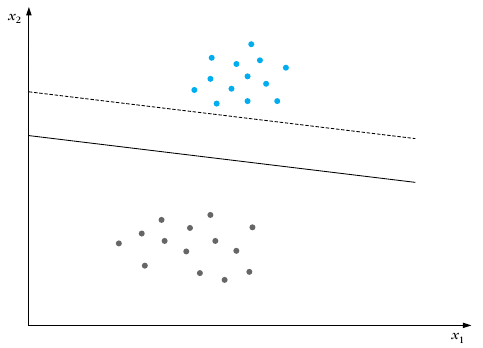
\includegraphics[scale=0.5]{img/linearniklasifikator.png}
\caption{Prikaz  dviju mogućih hiperravnina između dva razreda.}
\end{figure}

Slika 2.11 preuzeta iz \citep{pattern}. Obje 
hiperravnine mogu poslužiti za odjeljivanje prikazanih razreda, međutim, 
uvijek je poželjnije imati čim otporniji klasifikator. Značenje otpornosti je u 
sljedećem. Ako se pojavi neki vektor koji je imalo ispod crtkane linije, 
klasificira se kao razred sivih točaka iako to ne bi bio slučaj malo pomnijim 
gledanjem slike. Cilj klasifikatora je izgraditi hiperravninu koja odjeljuje dva 
razreda, ali istovremeno ta hiperravnina mora biti što udaljenija od oba razreda 
čime se postiže otpornost klasifikatora na vektore koji malo odskaču od svojih razreda, 
bilo radi neke vrste šuma ili čega drugoga. 

\bigbreak

Svaka hiperravnina je određena svojim smjerom (određeno s \textit{w}) i mjestom u prostoru (određeno s \(w_0\)). 
Pošto ne bismo željeli favorizirati niti jednu ravninu, trebamo odabrati jednu koja je 
jednako udaljena od odgovarajućih najbližih točaka razreda \(\omega_1\) i \(\omega_2\).  Odabrane hiperravnine 
označene su crnim linijama na slici 2.12 (Preuzeta iz \citep{pattern}). Margina udljenosti 1 je 2\(z_1\), a udaljenosti 2 je 2\(z_2\). 
Cilj je pronaći smjer koji daje maksmalnu moguću marginu. Margina je najmanja udaljenost 
između nekog vektora \(x_i\) i hiperravnine.

%slika s granicama
\begin{figure}[htbp]
\centering
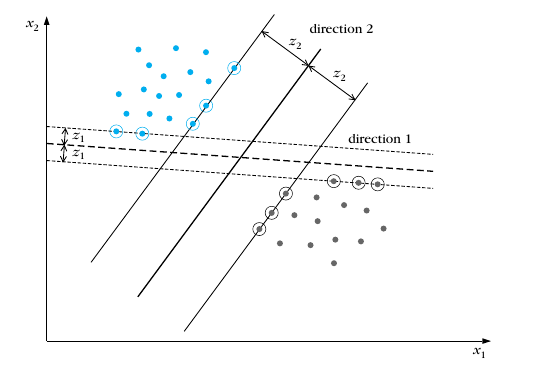
\includegraphics[scale=0.5]{img/slika10.png}
\caption{Prikaz potencijalnih hiperravnina koje dijele najbliže točke razreda}
\end{figure}

\newpage

Želimo postići da je vrijednost \(g(x)\) u blizini najbliže točke jednaka 1 za razred \(\omega_1\), a
-1 za razred \(\omega_2\) što je moguće zapisati na sljedeći način

\begin{equation}
y_i(w^Tx_i + w_0) \ge 1, i = 1,2,...,N
\end{equation}

Kako bi dobili udaljenost dviju margina uzmimo jedan vektor \(x_p\) koji označava 
vektor iz središta koordinatnog sustava do neke točke na margini plavih točaka i 
drugi vektor \(x_s\) koji označava vektor iz središta koordinatnog sustava do neke točke 
na margini sivih točaka. Razlika tih dvaju vektora je vektor \(v_{ps}\). Umnožak vektora 
\(v_{ps}\) i jediničnog vektora dao bi udaljenost između dviju margina. Kako bi dobili 
jedinični vektor možemo podijeliti vektor  njegovom apsolutnom vrijednošću \(\left| \left| w \right| \right|\). 

\bigbreak

Umnoškom vektora \(v_{ps}\) i jediničnog vektora dobiva se \(\frac{2}{\left| \left| w \right| \right|}\).
Kako bi maksimizirali udaljenost između margina, moramo minimizirati \(\left| \left| w \right| \right|\). 
Kao funkciju minimizacije uzimamo \(\frac{1}{2}\left| \left| w \right| \right|^2\) radi dobrih matematičkih
svojstava. Za pronalazak minimuma uz ograničenja (1) možemo koristiti Lagrangeove multiplikatore. 



Funkcija optimizacije se pretvara u

\begin{equation}
L = \frac{1}{2}\left| \left| w \right| \right|^2 - \sum_i \alpha_i \left[y_i \left(w \cdot x_i + w_0\right) - 1\right]
\end{equation}

Za dobivanje ekstrema (2.2) potrebno je derivirati i izjednačiti s 0.

\[
\frac{\partial L}{\partial w} = w - \sum_i \alpha_i y_i x_i = 0
\]

\begin{equation}
w = \sum_i \alpha_i y_i x_i
\end{equation}

\[
\frac{\partial L}{\partial w_0} = w - \sum_i \alpha_i y_i = 0
\]

\begin{equation}
\sum_i \alpha_i y_i = 0
\end{equation}

\bigbreak

Uvrštavanjem (2.3) i (2.4) u (2.2) dobiva se sljedeći izraz

\begin{equation}
L = \sum_i \alpha_i - \frac{1}{2} \sum_i \sum_j \alpha_i \alpha_j y_i y_j x_i^T \cdot x_j
\end{equation}

uz uvjet

\[
\sum_i \alpha_i y_i = 0
\]

čime se dobiva krajnji izraz koji je potrebno maksimizirati po \(\alpha\) nekim optimizacijskim
algoritmom. Iz izraza je vidljivo da njegova maksimizacija ovisi o umnošku parova početnih uzoraka. 
Jednom kada se Lagrangeovi multiplikatori izračunati, optimalna hiperravnina se dobiva 
uvrštavanjem u (2.3). Prikazani postupak optimizacije vrijedi i daje dobre rezultate u slučaju 
kada su razredi linearno odvojivi, u slučaju kada nisu postupa se drugačijim pristupom problemu.

\begin{multicols}{2}
Slučaj kada razredi nisu linearno odvojivi prikazan je na slici 2.13. Koliko god se trudilil nikako 
nije moguće pravcem odijeliti dva razreda kako se ne bi događala kriva klasifikacija nekih 
budućih uzoraka. Ideja je prijeći u neki viši dimenzijski sustav u nadi da će razredi postati 
linearn odvojivi. Uzmimo kao primjer sliku 2.13. i prijeđimo u trodimenzionalni sustav. Novonastala 
situacija prikazana je na slici 2.14. U ovoj dimenziji granica koja dijeli razrede uzoraka 
postaje ravnina. Vidimo da je u prostoru s ovom dimenzionalnošću moguće odijeliti uzorke jedne 
od drugih tako da ne postoje preklapanja dvaju razreda koja bi rezltirala krivom klasifikacijom.
Granica koja dijeli dva razreda prikazana je zelenkastom bojom na slici 2.14.

\begin{minipage}{\linewidth}
\vspace{10pt}
\centering
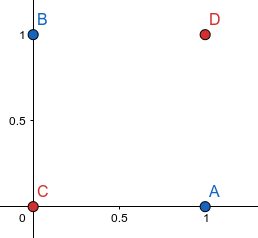
\includegraphics[width=0.8\linewidth]{img/neseparabilni.png}
\captionof{figure}{Linearno nerazdvojivi razredi}
\end{minipage}
\end{multicols}


\begin{minipage}{\linewidth}
\vspace{10pt}
\centering
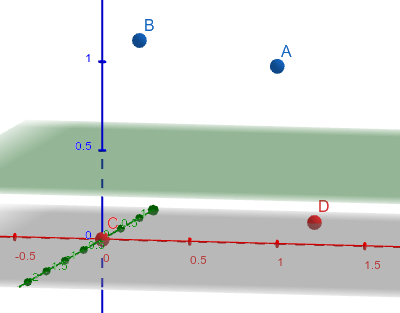
\includegraphics[width=0.7\linewidth]{img/3d.png}
\captionof{figure}{Linearno nerazdvojivi razredi u većoj dimenziji postaju linearno odvojivi}
\end{minipage}

\bigbreak

Funkcija kojom se prelazi u drugu dimenziju označava se s \(\varphi(x)\). Kako bi se navedena ideja
koristila u funkciji koja se maksimizira, dovoljno je samo napraviti sljedeće
jer funkcija ovisi samo o polaznom skupu uzoraka, odnosno \(X\).

\[
L = \sum \alpha_i - \frac{1}{2} \sum_i \sum_j \alpha_i \alpha_j y_i y_j \varphi(x_i) \cdot \varphi(x_j)
\]

Kraći zapis zapis korišten za \(\varphi(x_i) \cdot \varphi(x_j)\) je \(k(x_i, x_j)\) čime se označavaju 
jezgrene funkcije. Jezgrene funkcije služe za preslikavanje uzoraka iz početne, relativno niske 
dimenzionalnosti, u višu, moguće puno veću dimenzionalnost od izvorne kako bi uzorci u višoj 
dimenzionalnosti bili linearno odvojivi.

\begin{table}[htbp]
\centering
\caption{Prikaz nekih popularnih jezgara}
\begin{tabular}{ll}
\hline
ime & formula \\ \hline
Linearna: & \(K\left( x_i, x_j\right) = x_i^Tx_j\) \\
Polinomna: & \(K\left( x_i, x_j\right) = \left( a \cdot x_i^Tx_j + b\right)^d\)  \\
RBF: & \(K\left( x_i, x_j\right) = e^{-\frac{\left\lVert x_i - x_j \right\rVert^2}{\sigma^2}}\) \\
Sigmoida: & \(K(x_i, x_j) = tanh\left( \sigma x_i^T x_j + r\right)\) \\
Potencija: & \(K\left( x_i, x_j\right) = -\left\lVert x_i - x_j\right\rVert^\beta\) \\
Logaritam: & \(K\left( x_i, x_j\right) = -log\left( 1 + \left\lVert x_i - x_j\right\rVert^\beta\right)\) 
\end{tabular}
\end{table}

\newpage

Ova inačica SVM-a namijenjena je klasifikaciji gdje samo postoje 2 razreda. Međutim, 
jedan problem s više razreda može se podijeliti u više manjih binarnih problema klasifikacije. 
Popularne metode su: 

\begin{itemize}
	\item jedan protiv svih gdje se labela uzorku dodijeljuje prema klasifikatoru koji 
	ima funkciju najveće vrijednosti 
	\item jedan protiv drugog gdje se uzorak klasificira prema strategiji najvećeg 
	broja pobjedi što znači da svaki od klasifikatora pridjeljuje pripadnost jednom od razreda i razred s najviše glasova pobjeđuje
\end{itemize}

Pojam stroja s potpornim vektorima javlja se već sredinom 60-ih godina prošlog stoljeća od strane
Vladimira Vapnika čija ideja u tašnje vrijeme nije najbolje prihvaćena. Tek se 1990.-ih daje 
veća pažnja i uviđa potencijal SVM-a. Na slici 2.15 prikazan je jedan SVM sustav koji se koristio s
neronskim mrežama, a bio je pod nazivom \enquote{mreža s potpornim vektorima}.

\begin{minipage}{\linewidth}
\vspace{10pt}
\centering
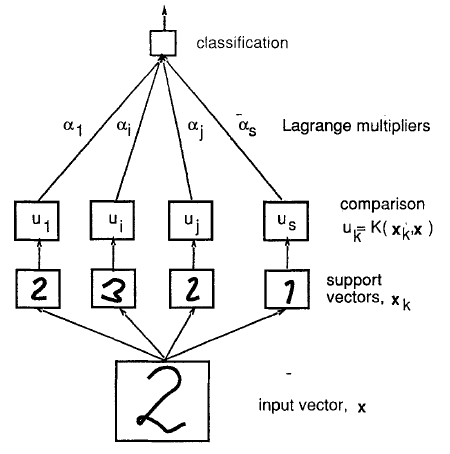
\includegraphics[width=0.7\linewidth]{img/svmnn.png}
\captionof{figure}{Prikaz mreže s potpornim vektorima}
\end{minipage}

\bigbreak

Jednom neshvaćena ideja se danas koristi u širokom spektru problema i predstavlja relativno
jednostavan alat u borbi s kategorizacijskim problemima. Slika 2.15 preuzeta iz \citep{vapnik}.


\newpage

\subsection{Gradijent slike}

Gradijent slike je promjena intenziteta ili boje u nekom smjeru na slici.

\begin{figure}[htbp]
\centering
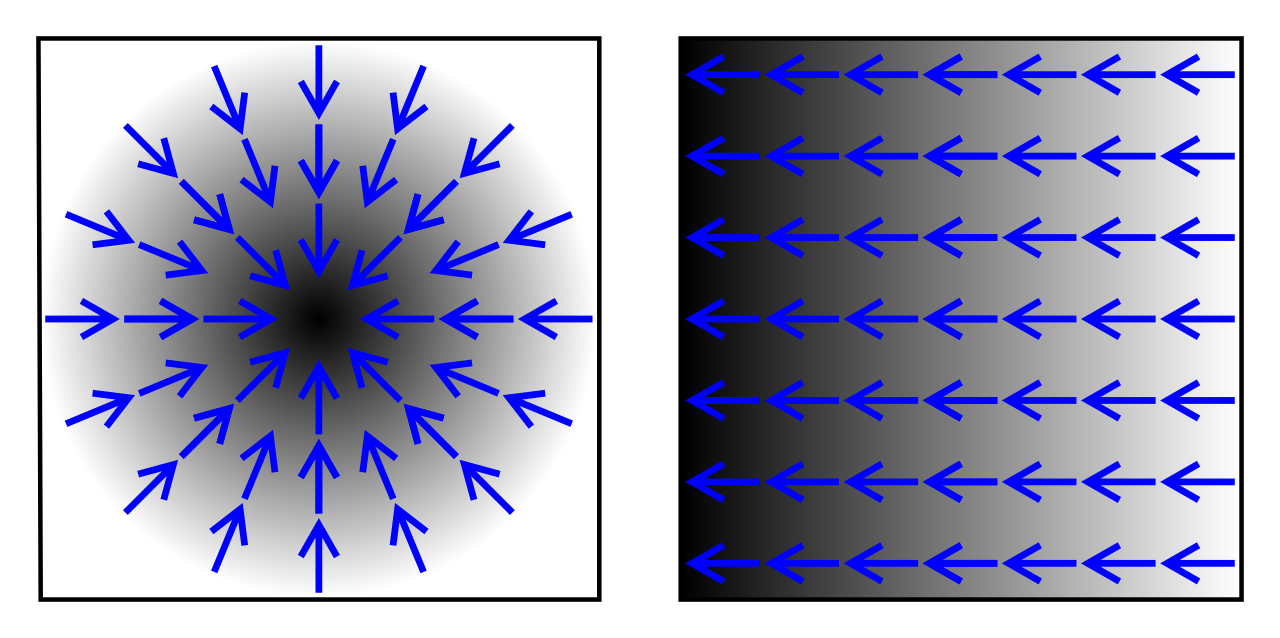
\includegraphics[width=0.8\linewidth]{img/Gradient2.png}
\caption{Prikaz smjera gradijenta plavim strelicama, tamnija boja označava veće vrijednosti.}
\end{figure}

Matematički, gradijent je funkcija dviju varijabli, vektor s dvije komponente koje su dobivene
derivacijom u horizontalnom i vertikalnom smjeru. Na svakom pikselu vektor gradijenta je smjer 
najveće promjene intenziteta, a duljina toga vektora odgovara brzini promjene u tom smjeru.

\[
\nabla f = \left[ \begin{array}{c} g_x \\ g_y \end{array}\right]
 = \left[ \begin{array}{c} \frac{\partial f}{\partial x} \\ \frac{\partial f}{\partial y} \end{array}\right]
 \textrm{, a iznos je dan s  } \sqrt{g_x^2 + g_y^2}
\]

\bigbreak

Kako je funkcija intenziteta slike pozanta samo u diskretnim točkama, derivacija ove funkcije 
ne može biti definirana ako se ne pretpostavi da iza svega toga leži kontinuirana funkcija 
intenziteta koja je uzorkovana u nekim konkretnim pikselima. Aproksimacije ovih funkcija derivacije 
mogu biti definirane s različitim stupnjevima točnosti. Jedan od popularnih načina za 
aproksimaciju gradijenta slike je konvolucija slike s nekom jezgrom, primjerice sa Sobelovim operatorom.
Slika 2.16 preuzeta iz \citep{wikiGradient}.

\newpage

\subsection{Sobelov operator}

Ovaj operator koristi dvije 3 \(\times\) 3 jezgre koju su konvolirane s izvornom slikom kako bi se aproksimirale 
derivacije – jedna za x smjer, a druga za y smjer. Označimo izvornu sliku kao dvodimenizonalnu matricu \(A\), sliku
koja je dobivena konvolucijom jezgre za x smjer i slike \(A\) kao \(G_x\), a sliku koja je dobivena konvolucijom 
jezgre za y smjer i slike \(A\) s \(G_y\).

\[G_x = 
\begin{bmatrix} 
1 & 0 & -1\\ 
2 & 0 & -2\\ 
1 & 0 & -1 
\end{bmatrix}
 * A
  \quad\quad\quad
 G_y = 
\begin{bmatrix} 
 1 & 2 & 1\\ 
 0 & 0 & 0\\ 
 -1 & -2 & -1
\end{bmatrix}
 * A
\]
\bigbreak
gdje * označava operaciju konvolucije, a krajnja slika se dobije na sljedeći način 
\[
G = \sqrt{G_x^2 + G_y^2}
\].

\underline{\textbf{Primjer} - Izgled izračuna Sobelovog operatora}

\begin{multicols}{2}

\begin{minipage}{\linewidth}
\centering
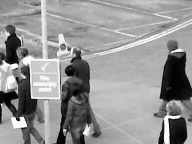
\includegraphics[width=0.8\linewidth]{img/2982.jpg}
\captionof{figure}{Izvorna slika}
\end{minipage}

\begin{minipage}{\linewidth}
\centering
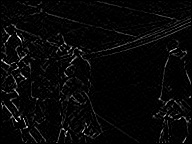
\includegraphics[width=0.8\linewidth]{img/sobel.jpg}
\captionof{figure}{Primijenjen Sobelov operator na izvornoj slici}
\end{minipage}

\begin{minipage}{\linewidth}
\centering
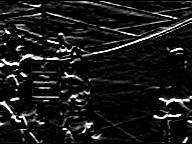
\includegraphics[width=0.8\linewidth]{img/sobely.jpg}
\captionof{figure}{Primijenjen Sobelov operator u smjeru y na izvornoj slici}
\end{minipage}

\begin{minipage}{\linewidth}
\centering
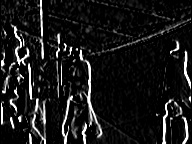
\includegraphics[width=0.8\linewidth]{img/sobelx.jpg}
\captionof{figure}{Primijenjen Sobelov operator u smjeru x na izvornoj slici}
\end{minipage}

\end{multicols}

\newpage

\subsection{Haralickove značajke}

Početna pretpostavka u karakterizaciji teksture slike je da 
matrica pojavnosti sivih razina sadrži svu  informaciju o teksturi slike. 
Samim time sve teksturne značajke će se izračunavati iz matrice pojavnosti sivih 
razina. Funkcije koje definiraju skup od 14 mjera teksturnih značajki dane su u dodatku A. 
Neke od tih mjera se odnose na specifične teksturne karakteristike poput homogenosti, 
kontrasta i prisutnosti grupiranih ili usmjerenih struktura unutar slike. Druge mjere 
opisuju složenost i način promjene sivih razina unutar slike.

\bigbreak

Postoje neka intuitivna očekivanja u pogledu svojstava koja se odnose na neke značajke.
Primjerice, bilo bi za očekivati da će vrijednost entropije poprimati veće vrijednosti za složenije slike. 
Možda bi također bilo moguće uočiti neke linearne zavisnosti u slikama koje imaju velike 
vrijednosti funkcije korelacije.

\bigbreak

Utjecaj na vrijednosti Haralickovih značajki uvelike ima i veličina slike nad kojom se konstruira
GLCM te iz koje se izračunavaju i same značajke. Ukoliko slika nije dovoljno velika, neće sadržavati
dovoljno teksturnih informacija koje su zaslužne za razlikovanje različitih područja interesa dok s druge
strane prevelika slika može sadržavati više različitih razreda ili regija koje pokušavamo odvojiti i razlikovati.

\bigbreak

Iako te mjere sadrže informaciju o teksturnim značajkama slike, teško je identificirati koja je teksturna 
značajka karakterizirana nekom konkretnom funkcijom. Definicije funkcija iz dodatka A
preuzete su iz izvornog rada Haralicka i drugih \citep{haralick}.

\chapter{Opis postupka}

Predlaže se tehnika klizećeg okna za klasifikaciju i lociranje područja
mnoštva. Pripremne radnje obuhvaćaju pretvorbu izvornih slika, dimenzija
768 x 576, u sive razine i dijeljenje njih samih u manje podslike, dimenzija
192 x 144, kojih ima 16 po svakoj izvornoj slici. Svaka podslika razlikuje se 
po gustoći mnoštva, pozadini i uvjetima osvjetljenja.  

\begin{figure}[ht]
	\begin{subfigure}[b]{0.19\linewidth}
		\centering
		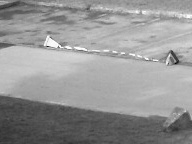
\includegraphics[scale=0.5]{img/noflow.jpg}
		\caption{No flow}
	\end{subfigure}
	\begin{subfigure}[b]{0.19\linewidth}
		\centering
		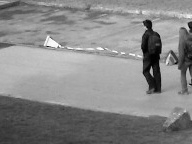
\includegraphics[scale=0.5]{img/freeflow.jpg}
		\caption{Free flow}
	\end{subfigure}
	\begin{subfigure}[b]{0.19\linewidth}
		\centering
		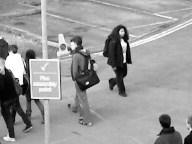
\includegraphics[scale=0.5]{img/restrictedflow.jpg}
		\caption{Restricted flow}
	\end{subfigure}
	\begin{subfigure}[b]{0.19\linewidth}
		\centering
		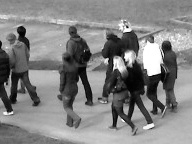
\includegraphics[scale=0.5]{img/denseflow.jpg}
		\caption{Dense flow}
	\end{subfigure}
	\begin{subfigure}[b]{0.19\linewidth}
		\centering
		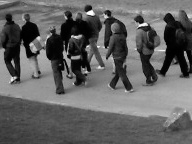
\includegraphics[scale=0.5]{img/jammedflow.jpg}
		\caption{Jammed flow}
	\end{subfigure}
\caption{Prikaz pojedinih gustoća mnoštva}
\end{figure}

Sve se podslike ručno označe pripadnim razredima gustoće prema
\citep{polus} uz dodatnu oznaku \enquote{no flow} koja 
predstavlja podslike u kojima nema nikakvog mnoštva. Sljedeće se primjenjuje
operator LBP nad svakom podslikom i pritom je potrebno napomenuti da
 postoje dvije vrste izračuna LBP operatora. Jedan se izračunava nad slikama 
sivih razina, a drugi nad slikama koje su također sivih razina, ali je nad njima 
primijenjen operator gradijenta. Nakon dobivene slike lokalnih binarnih 
značajki, koristeći se tenhnikom kliznog okna, konstruira se matrica 
pojavnosti lokalnih binarnih značajki (LBPCM) nad svakim oknom podslike. 
Iz svake LBPCM izračunavaju se željene Haralickove značajke i te se vrijednosti
pohranjuju u vektor značajki. Vektor značajki se sastoji od vrijednosti
Haralickovih značajki svakog okna, odnosno vektor značajki neke podslike 
sastoji se od vrijednosti Haralickovih značajki njezinih okana. Po završteku 
stvaranja, vektori značajki, se predaju \textit{k}-NN klasifikatoru ili SVM-u.

\newpage

Na kraju se pristupa evaluaciji samih klasifikatora i eventualnoj izmjeni
samih parametara u nadi boljeg rezultata u sljedećoj iteraciji učenja. Za učenje
klasifikatora korisiti se \(70\%\) izvornih slika, a za testiranje ostatak.

\begin{figure}[!ht]
\centering
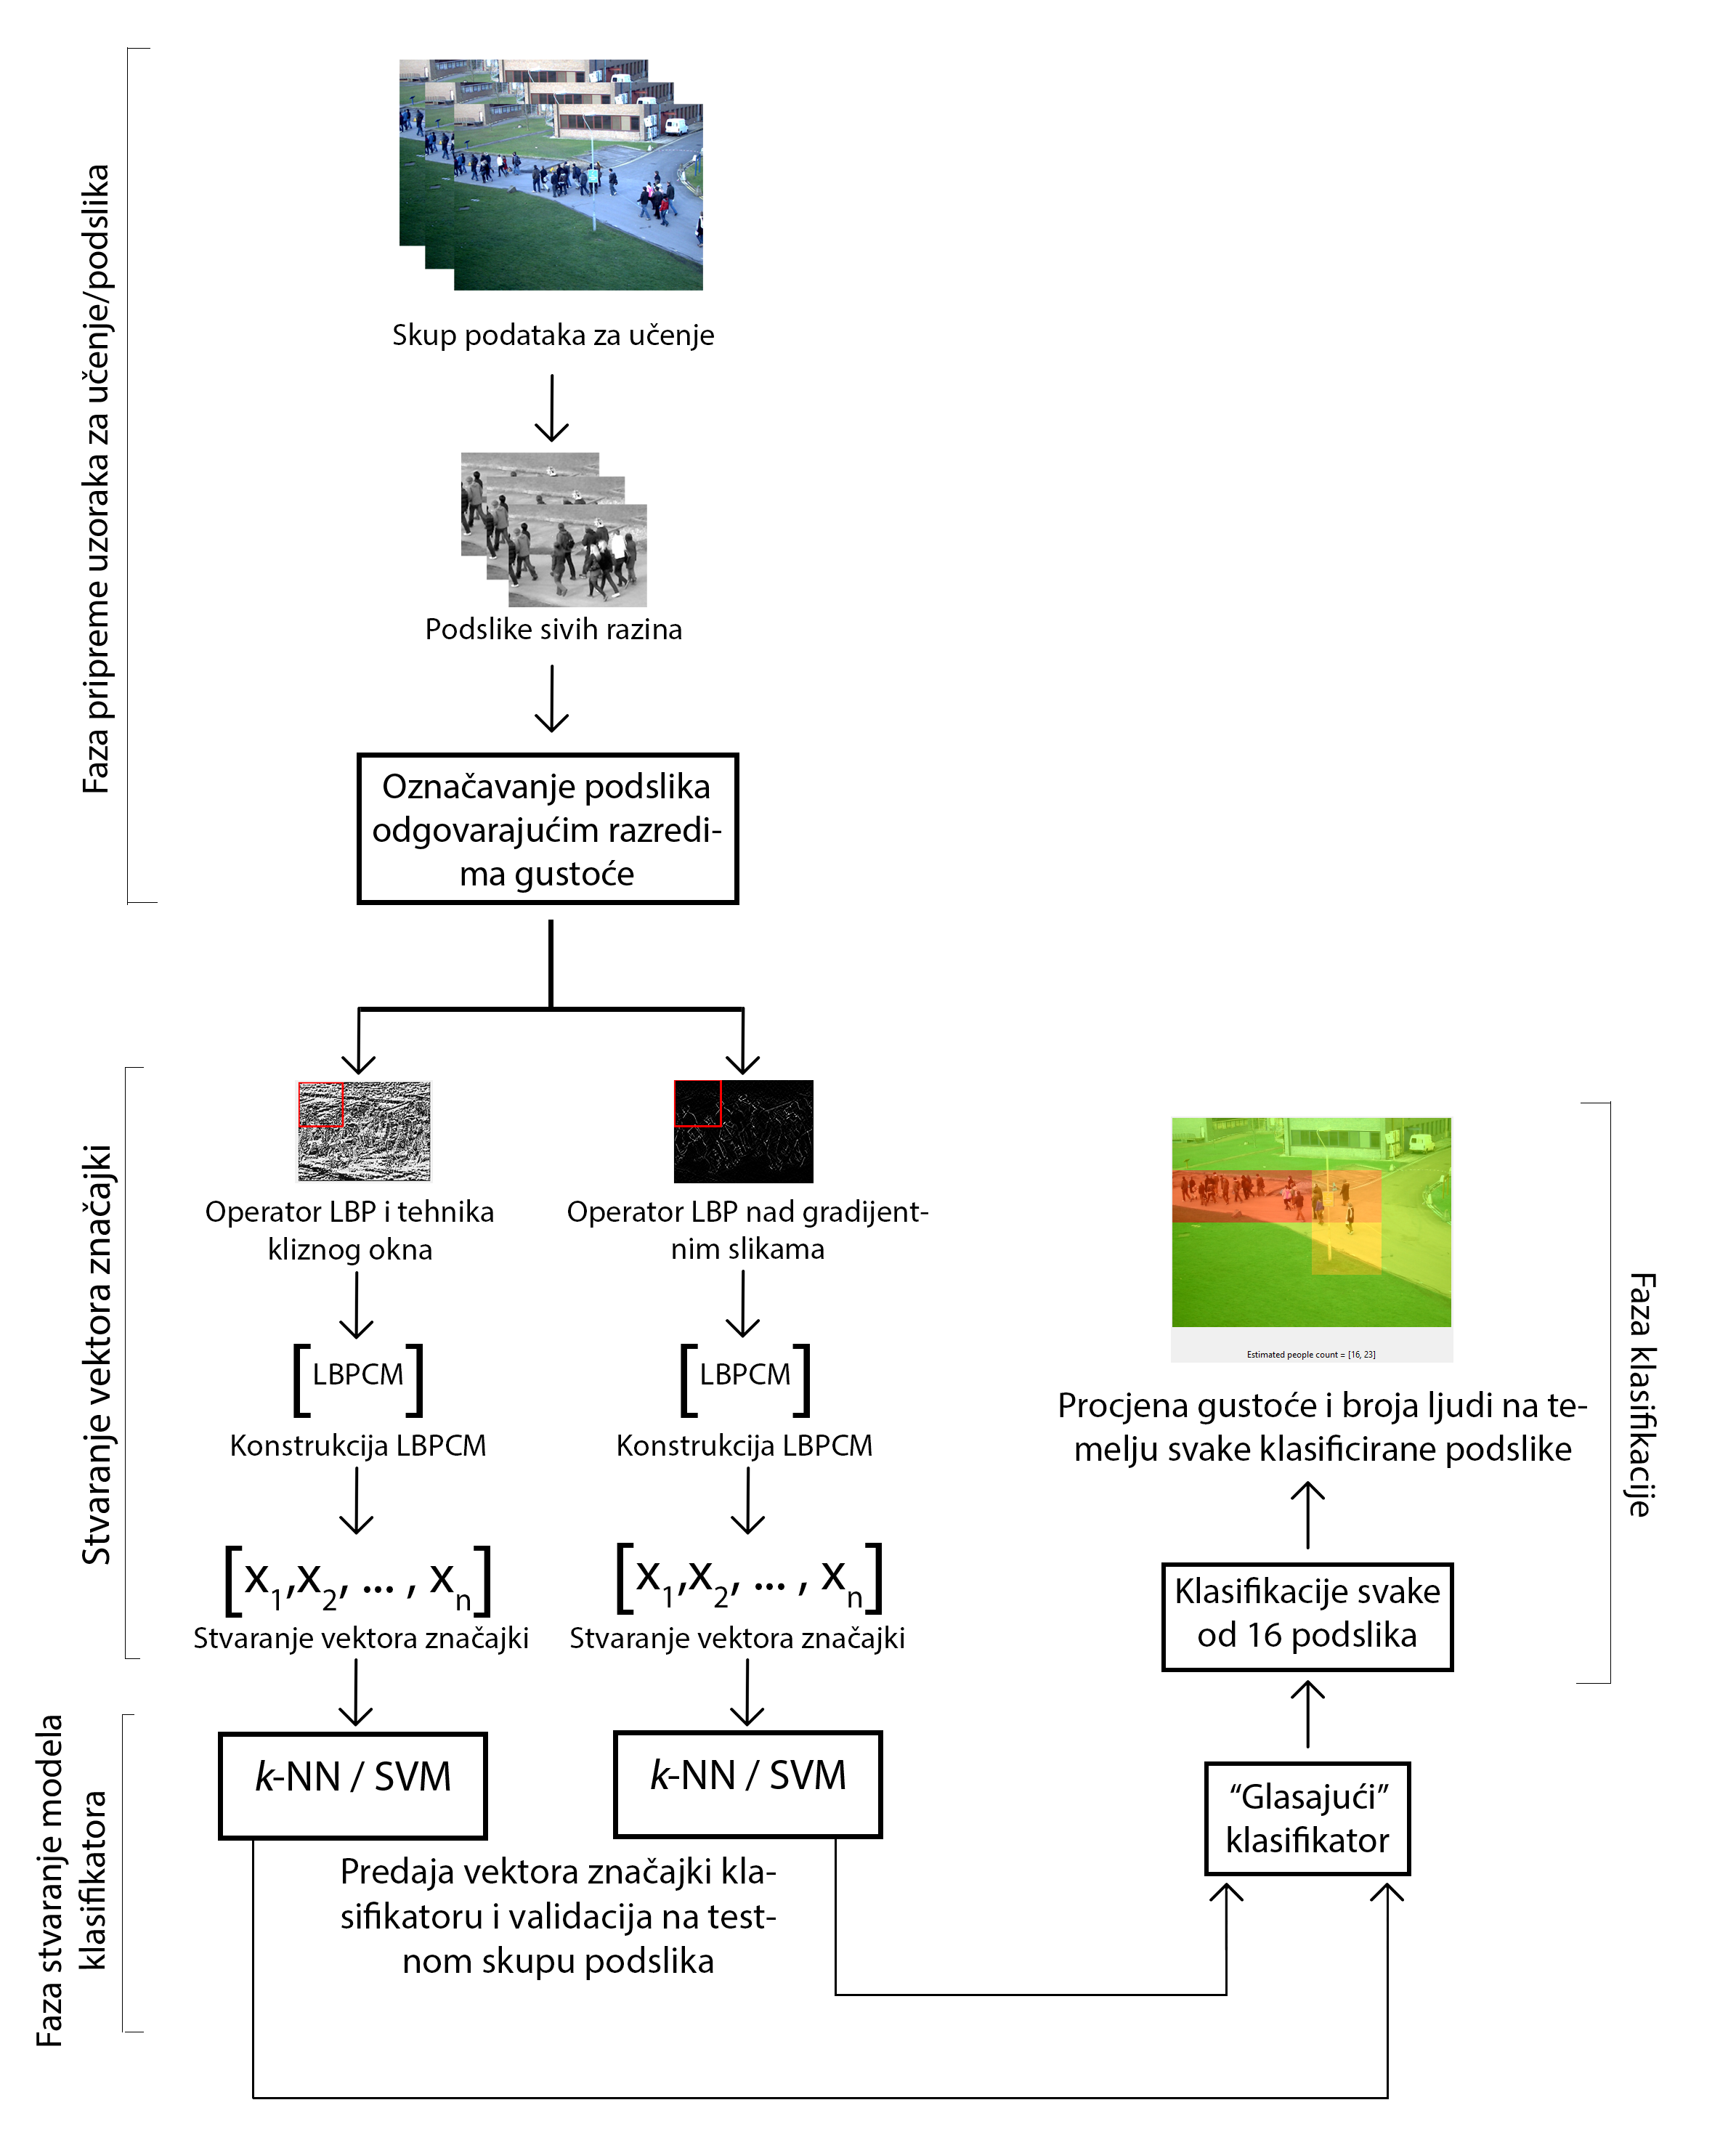
\includegraphics[scale=0.18]{img/somprobajzbrisati.png}
\caption{Prikaz arhitekture sustava}
\end{figure}

\newpage

Prethodno opisan postupak moguće je vidjeti na slici 3.2 gdje je
prikazana arhitektura sustava i pojedine faze koje su kasnije u poglavlju 4 
detaljnije opisane. Prva faza obuhvaća samu pripremu podslika koje se 
koriste za stvaranje vektora značajki. Nakon prve faze događa se grananje
u dva dijela: prvi dio obuhvaća klasifikatore koji koriste slike sivih razina 
nad kojima se primjenjuje operator LBP, dok drugi dio predstavlja klasifikatore
koji koriste slike sivih razina nad kojima se primjenjuje operator gradijenta
i tek nakon toga operator LBP. Nakon što su dobiveni vektori značajki 
svakog, oni se prosljeđuju odgovarajućem klasifikatoru kako bi se izvršila
ocjena njihove točnosti, odnosno validacija na testnom skupu podataka.
Jednom kada su ocijenjeni klasifikatori moguće je napraviti prividnu 
fuziju u jedan klasifikator.

\bigbreak

Sjedinjenje dvaju različitih klasifikatora obavlja se pomoću nove vrste
klasifikatora - glasačkog klasifikatora (engl. \textit{voting classifier}).
Poželjno je da se koristi jedan koji koristi slike sivih razina, a jedan 
slike nad kojima je primijenjen operator gradijenta kako bi tako
stvoren klasifikator bio robusniji te dao potencijalno bolji rezultat.
Ovakva vrsta klasifikatora pogodna je zbog načina na koji daje važnost pojedinim
klasifikatorima od kojih se sastoji. 

\bigbreak

Na odluku klasifikatora može se utjecati
na više načina. Prvi je \enquote{tvrdo glasanje} (većinsko glasanje), gdje
svaki od klasifikator glasa za neku labelu, a najbrojnija labela pobjeđuje 
i dodjeljuje se novome uzorku koji se klasificira. Ovakvo glasanje je moguće i 
modificirati na način da se svakome klasifikatoru dodijeli neka težina, 
npr. ovisno o točnosti njegove klasifikacije na setu slika za učenje.

\bigbreak

Drugi način je \enquote{meko glasanje} (engl. \textit{soft voting}) gdje
se dohvate vjerojatnosti klasifikacije svake labele svakog od klasifikatora,
uprosječe se, pa se na temelju tih novih vjerojatnosnih vrijednosti određuje
pripadnost dosad neviđenog uzorka. Pošto su poznate vjerojatnosti klasifikacije
moguće je množiti svaku vjerojatnost nekom težinom i time utjecati na ishod odluke.

\bigbreak

Odabrana je druga vrsta glasanja, tzv. \enquote{meko glasanje} jer je eksperimentom
utvrđeno da daje bolje rezultate nad skupom podataka koji se koristi u radu.  

\newpage

\underline{\textbf{Primjer} - Dobivanje vjerojatnosti glasačkog klasifikatora}

\[y = \argmax_i \sum_{j=1}^mw_jp_{ij}\]

gdje \(w_j\) predstavlja težinu pridijeljenu \(j\)-tom klasifikatoru.

\bigbreak

Uzmimo 3 klasifikatora i dva moguća razreda pripadnosti svakog uzorka 

\begin{center}
\(C_1(x) \rightarrow [0.9,0.1]\),
\end{center}
\begin{center}
\(C_2(x) \rightarrow [0.8,0.2]\),
\end{center}
\begin{center}
\(C_3(x) \rightarrow [0.4,0.6]\)
\end{center}

Koristeći uniformne težine dobivamo sljedeće srednje vjerojatnosti (\(i_0\) i \(i_1\) predstavljaju razrede):
\begin{center}
\(p(i_0|x)=\frac{0.9+0.8+0.4}{3}=0.7\)

\(p(i_1|x)=\frac{0.1+0.2+0.6}{3}=0.3\)

\(y=\argmax_i [p(i_0|x),p(i_1|x)]=0\)
\end{center}

Promjenimo iznose težina svakog klasifikatora sljedećim \(\{0.1,0.1,0.8\}\). Sada izračun
vjerojatnosti izgleda na sljedeći način

\begin{center}
\(p(i_0|x) = 0.1 \cdot 0.9 + 0.1 \cdot 0.8 + 0.8 \cdot 0.4 = 0.49\)

\(p(i_1|x) = 0.1 \cdot 0.1 + 0.2 \cdot 0.1 + 0.8 \cdot 0.6 = 0.51\)

\(y=\argmax_i [p(i_0|x),p(i_1|x)]=1\)
\end{center}

Iz primjer je jasno vidljivo koliku važnost imaju pridijeljene težine svakom od
klasifikatora i ukoliko nisu ispravno dodijeljene, rezultat klasifikacije može
biti značajno lošiji od svakog pojedinog klasifikatora.



\chapter{Upute za korištenje i prikaz međukoraka}

Programska podrška ovdje obrađivanog postupaka pisana je u Python 3.6 
programskom jeziku. Usto je potrebno instalirati dodatne Python 
knjižnice: OpenCV \citep{opencv.org}, scikit-learn \citep{scikit} i PIL \citep{pil}.
OpenCV koristi se za učitavanje slika i pretvorbu slika u boji u slike sivih tonova. Scikit 
daje implementaciju \textit{k}-NN i SVM klasifikatora kako i funkciju za generiranje 
GLCM pojedine slike. PIL je korišten za pretvrbu normalne slike u oblik koji 
se koristi u Tkinter biblioteci koja je korištena za grafičko sučelje same aplikacije.
Za Haralickove značajke nije korištena nikakva biblioteka nego je izračun svake implementiran
zasebno.

\bigbreak

Za pokretanje aplikacije putem grafičkog sučelja potrebno je kliknuti 
na app.py ili putem terminala upisati naredbu „python app.py“ iz 
vršnog direktorija projekta. Nakon što je aplikacija pokrenuta 
otvoren je sljedeći prozor. 

\bigbreak

Početni prozor prikazuje naziv rada \citep{6266412} na kojem se temelji ovaj završni rad, 
slikovni prikaz postupka lokalnih binarnih značajki i gumb \enquote{Main screen}
koji otvara stranicu s glavnim funkcionalnostima aplikacije. U podnožuju svakog
prozora nalazi se prazan prozor \enquote{Console window} koji ima ulogu
mjesta u koje se ispisuju važnije informacije poput upozorenja, eventualnih 
grešaka i rezultata izvođenja nekih drugih funkcija. Pritiskom na gumb \enquote{Main screen}
otvara se glavni prozor koji sadrži sve funkcionalnosti aplikacije.

\bigbreak

\begin{figure}[!ht]
\centering
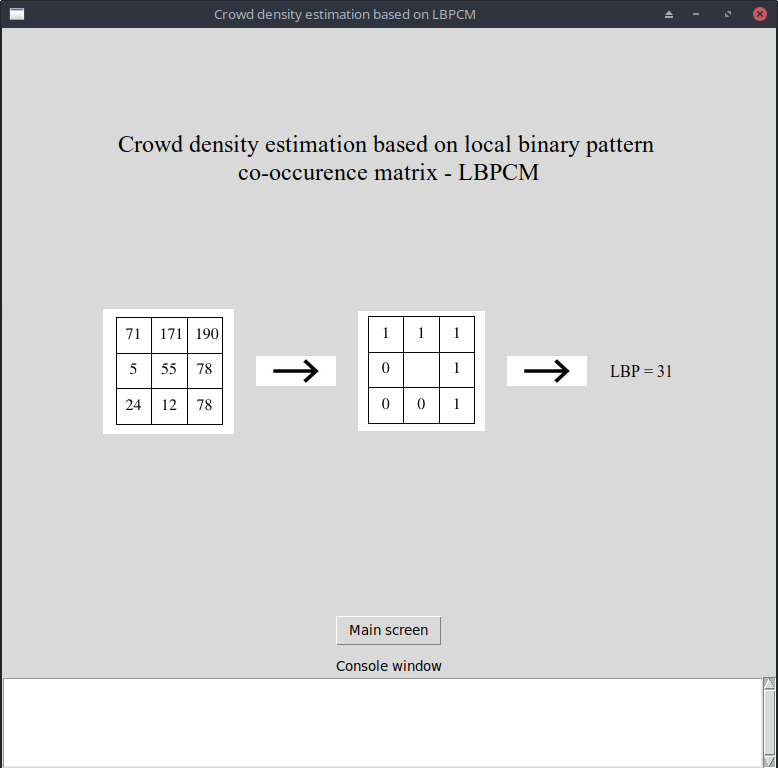
\includegraphics[scale=0.37]{img/startpage.png}
\caption{Prikaz početnog prozora nakon pokretanja aplikacije}
\end{figure}

\hfill

\begin{figure}[!ht]
\centering
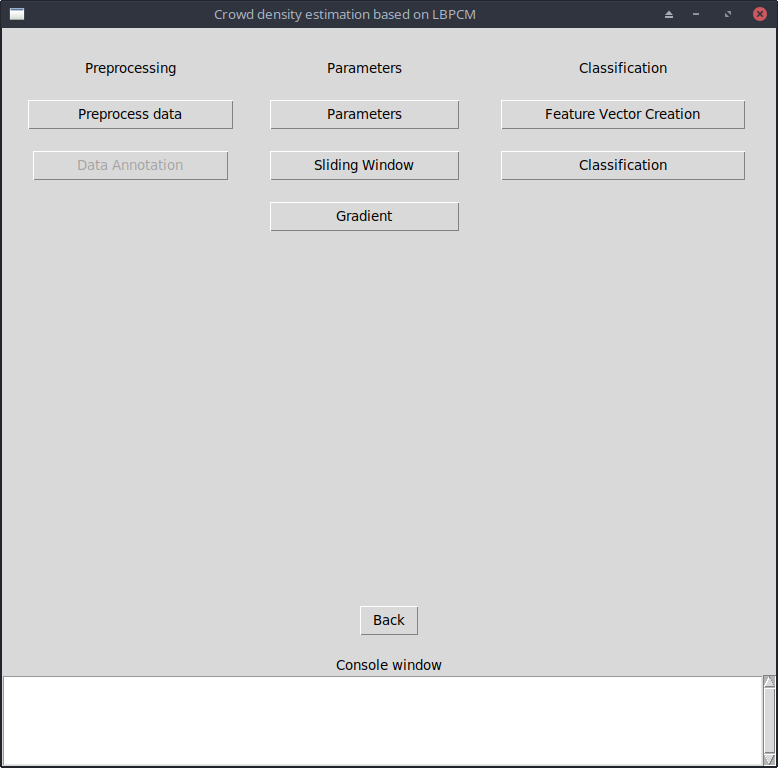
\includegraphics[scale=0.37]{img/mainscreen.png}
\caption{Prikaz glavnog prozora}
\end{figure}

Prostor glavnog prozora podijeljen je u tri dijela. Prvi dio se sastoji
od radnja koje je potrebno obaviti prije samog postupka učenja, a to su:
priprema izvornih slika podjelom u manje podslike i označavanje svake 
podslike odgovarajućim razredom gustoće mnoštva. Po završetku navedenih radnja
moguće je nastaviti s daljnjim postupkom.

\newpage

Drugi dio prozora služi za promjenu parametara aplikacije, uvid u tehniku 
klizećeg okna gdje je moguće vidjeti kako se mijenjaju iznosi Haralickovih značajki
prilikom putovanja klizećeg okna po pojedinoj slici i na kraju korištenje
opertora gradijenta na odabranoj slici.

\bigbreak

Zadnji dio prozora obuhvaća samu fazu stvaranja vektora značajki (učenje
klasifikatora) gdje se postavljaju svi parametri pojedinog modela te pokreće
postupak učenja i drugi dio koji je zaslužan za postupak klasifikacije
dosad neviđenih uzoraka nekim od već naučenih modela.


\subsection{Podjela slika u podslike}

Prije svega potrebno je pripremiti skup slika koji se koristi za učenje i 
kasnije za verifikaciju klasifikatora. Izvorni skup se sastoji od 221 slike (PETS2009 skup podataka)
koje su izvučene iz video zapisa jedne nadzorne kamere. Svaka slika je dimenzija
768 x 576 te se podijeli u 16 jednakih podslika 192 x 144. Ova konkretna dimenzija
podslika je odabrana kako ne bi ostalo neiskorištenih piksela na rubovima i 
kako dimenzija novonastalih podslika ne bi previše odskakala od veličine mnoštva
koje je prisutno u izvornim slikama. Nakon što su slike podijeljene na manje dijelove,
novonastalih podslika ima 3536 koje se zatim pretvaraju u slike sivih razina kako
bi se prilikom računanja Haralickovih značajki tijekom učenja klasifikatora taj
korak mogao preskočiti i time uštedjeti procesorsko vrijeme.

\begin{figure}[!ht]
\centering
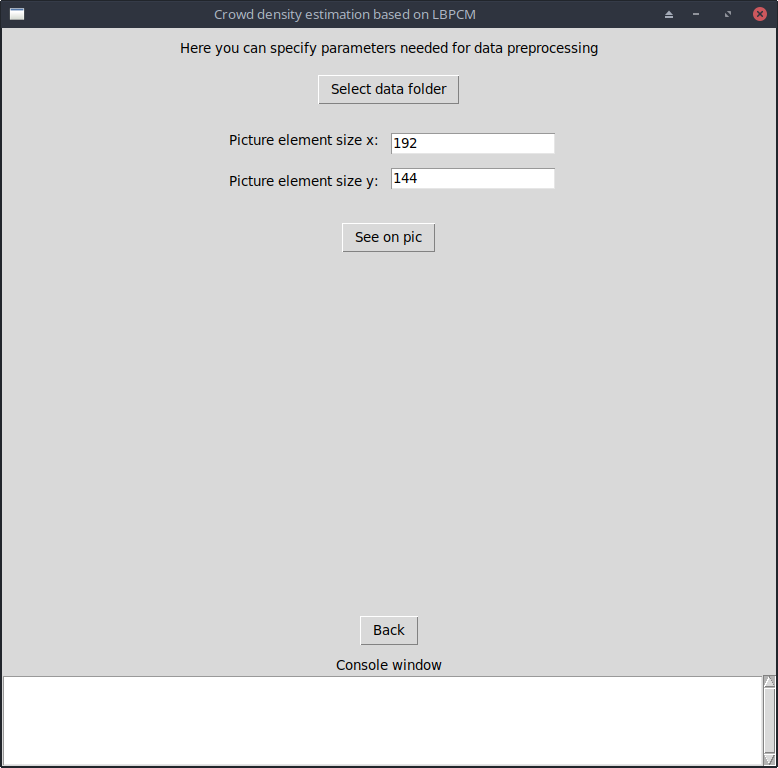
\includegraphics[scale=0.37]{img/preprocessdata.png}
\caption{Prikaz stranice za obradu izvornih slika}
\end{figure}

\bigbreak

Aplikacija nudi potporu za izvođenje navedenog postupka. Kako bi se izvorne
slike podijelile u manje podslike potrebno je pritisnuti na gumb \enquote{Preprocess data}
koji otvara stranicu izgleda na slici 4.3.

\bigbreak

Prozor na samom vrhu ima gumb za odabir direktorija koji sadrži izvorne slike
za učenje i testiranje. Po odabiru navedenog direktorija mogu se upisati 
željene dimenzije podslika koje će nastati dijeljenjem izvorne slike.
Prvi element unosa sadrži veličinu u x smjeru, a drugi u y smjeru. Nakon
unešenih dimenzija moguće je vidjeti kako bi izgledale konkretne dimenzije
na izvornoj slici pritiskom na gumb \enquote{See on pic}. Nakon pritiska na gumb
pojavljuje se sljedeći dio prozora.

\begin{figure}[!ht]
\centering
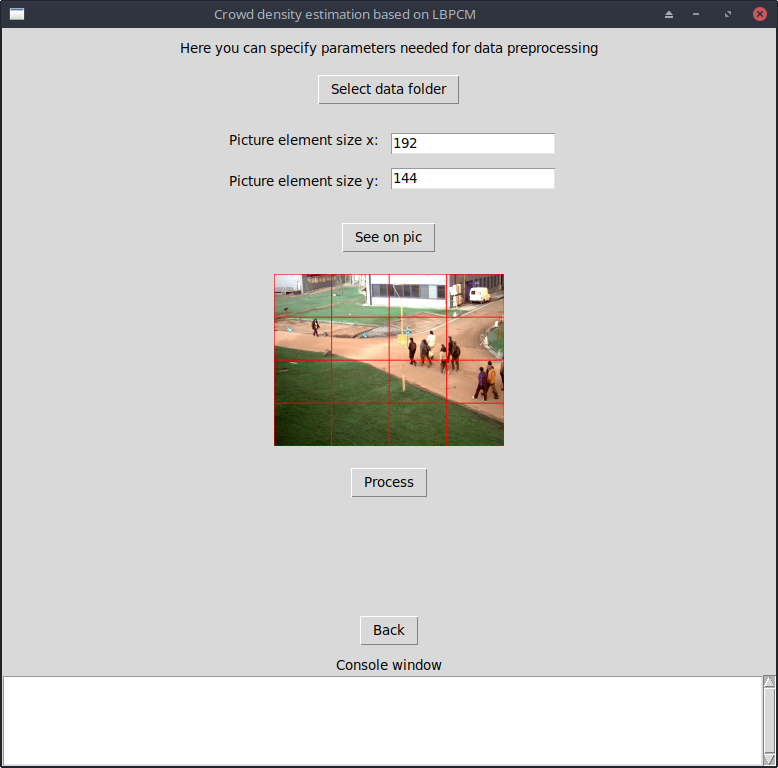
\includegraphics[scale=0.37]{img/seeonpic.png}
\caption{Prikaz izgleda podslike s unešenim dimenzijama}
\end{figure}

\bigbreak

Novi dio prozora prikazuje jednu izvornu sliku iz odabranog direktorija
s podjelom na manje podslike, a one su dimenzija unešenih iznad. Svaka podslika
prikazana je crvenim linijama i ako nismo zadovoljni njihovom dimenzijom
moguće je upisati neke druge vrijednosti i vidjeti novi rezultat. Ukoliko 
nam odgovara veličina podslika potrebno je pritisnuti gumb \enquote{Preprocess}
koji pokreće postupak dijeljenja slika iz odabranog direktorija i zapisuje ih u 
direktorij \enquote{preprocessedData}. Taj direktorij nakon završenog postupka
sadrži 3536 podslika u sivim razinama, ukoliko su korištene dienzije 192 x 144, 
pa je moguće prijeći u u sljedeću fazu, a to je označavanje svake pojedine podslike.

\begin{figure}[ht]
\centering
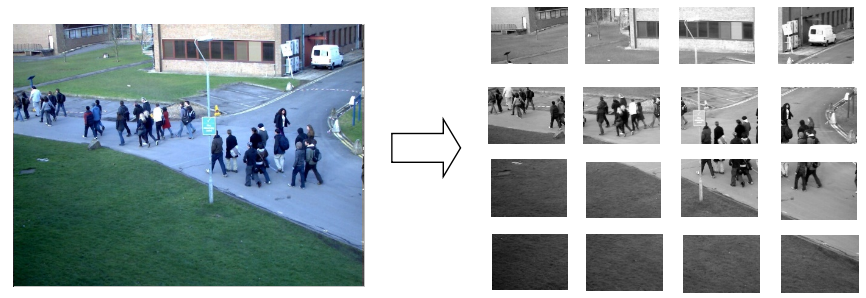
\includegraphics[scale=0.4]{img/splitted.png}
\caption{Prikaz podijeljene izvorne slika na manje podslike}
\end{figure}

\subsection{Označavanje podslika}

Po završetku dijeljenja izvornih slika u manje podslike pristupa se postupku
označavanja podslika. Kako bi mogli označiti svaku pojedinu podsliku na
što jednostavniji način potrebno je pritisnuti gumb \enquote{Data Annotation} 
u glavnom prozoru aplikacije. Nakon pritiska na gumb otvara se sljedeći prozor.

\begin{figure}[ht]
\centering
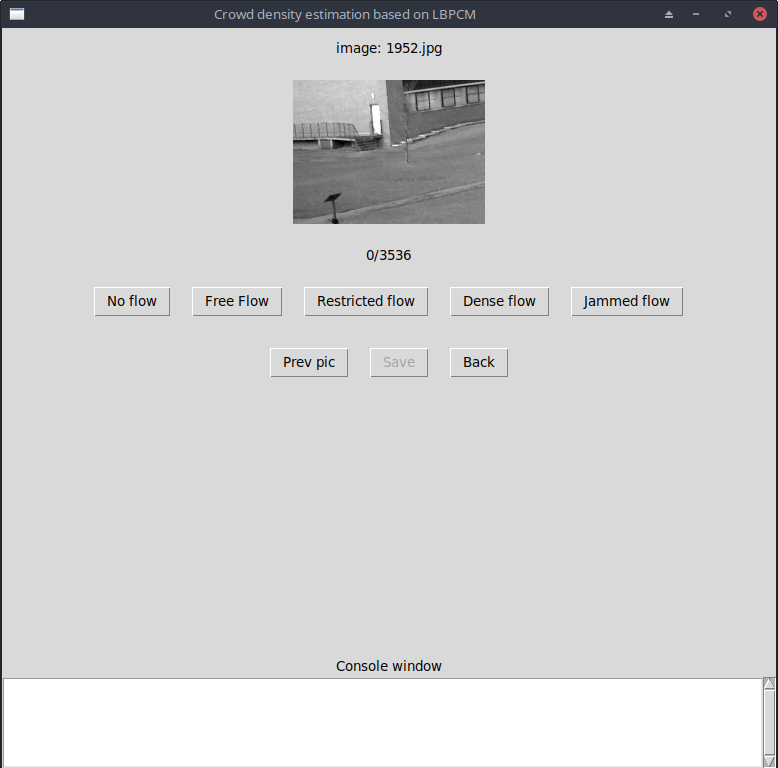
\includegraphics[scale=0.38]{img/dataannotation.png}
\caption{Prikaz prozora za označavanje podslika}
\end{figure}

Najgornji dio prozora prikazuje ime trenutne podslike koju je potrebno označiti.
Ispod naziva se nalazi konkretna slika koja se označava, a prisutan je i brojač
koji prikazuje broj označenih podslika. Ispod brojača postoji 5 gumba koji
označavaju razine gustoće mnoštva. Podslika se označava pritiskom na jedan
od gumba koji odgovara gustoći mnoštva zatečenoj na trenutnoj podslici. Nakon pritiska
na gumb pojavljuje se sljedeća od podslika koju je potrebno označiti, a labela
prethodne podslike se zapisuje u interni spremnik. 

\bigbreak

Nakon što su sve podslike označene
odgovarajućim labelama, interni spremnik je moguće spremiti na disk u obliku 
tekstualne datoteke pritiskom na gumb \enquote{Save}. Nakon pritiska na gumb
\enquote{Save} stvara se tekstualna datoteka imena \enquote{labeledData.txt}
, a svaki redak je oblika 0.jpg:2, gdje 0.jpg predstavlja ime podslike koje 
je jedinstveno, a 2 označava pripadni razred gustoće mnoštva. Ukoliko je 
došlo do pogreške prilikom označavanje neke podslike moguće je pritisnuti
gumb \enquote{Prev pic} čime se vraća prethodna slika kojoj je moguće pridijeliti
drugačiju labelu. Potrebno je napomenuti da se jednom označene podslike ne trebaju 
više označavati prilikom svakog procesa učenja nekog klasifikatora nego 
je samo potrebno učitati postojeću datoteku.

\subsection{Stvaranje vektora značajki}

Jednom kada se slike podijeljene u manje podslike i nakon završetka označavanja
svih podslika, moguće je pristupiti postupku stvaranja vektora značajki. 
Kako bi pristupili tome prozoru, potrebno je pritisnuti gumb \enquote{Feature Vector Creation} 
nakon čega se otvara prozor prikazan na slici 4.7.

Prozor ne prikazuje puno osim broja podslika i informacije jesu li labele
podslika učitane u memoriju ili nisu. Kako bi ih učitali potrebno je pritusnuti
na gumb \enquote{Load labels} nakon čega se otvara prozor za odabir tekstualne datoteke
s labelama. Ako su labele uspješno učitane, mijenja se tekst ispod broja
podslika u tekst zelene boje \enquote{LOADED}. Podnožje prozora još sadrži gumb
za povratak na prethodnu stranicu i gumb za dodavanje novih konfiguracije koji će biti
ubrzo objašnjen. 

\bigbreak

Središnji dio prozora trenutno ne prikazuje ništa jer nije dodana niti jedna
konfiguracija. Jednom kada se doda nova konfiguracija, u središnjom dijelu
prozora stvori se traka napretka koja prikazuje koliko još ima do završetka 
te pojedine konfiguracije. Stvaranju vektora značajki prethodi stvaranje neke konfiguracije. Kako bi se 
stvorila nova konfiguracija potrebno je pritisnuti na gumb \enquote{Add configurations}.
Nakon pritiska na gumb otvara se prozor prikazan na slici 4.8.

\bigbreak

\begin{minipage}{\linewidth}
\centering
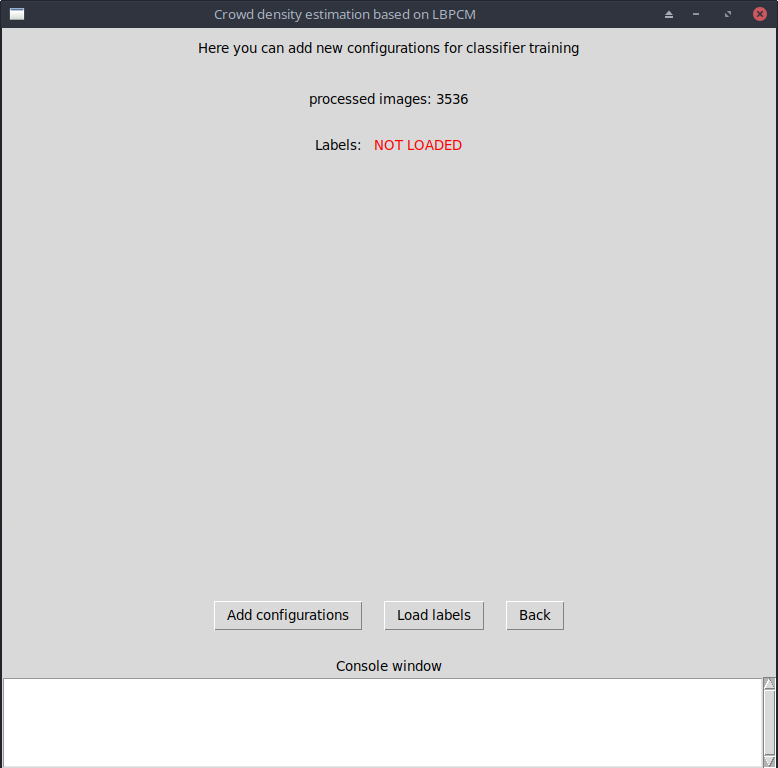
\includegraphics[scale=0.35]{img/fvc1.png}
\captionof{figure}{Početni prozor za stvaranje vektora značajki}
\end{minipage}

\bigbreak

\begin{minipage}{\linewidth}
\centering
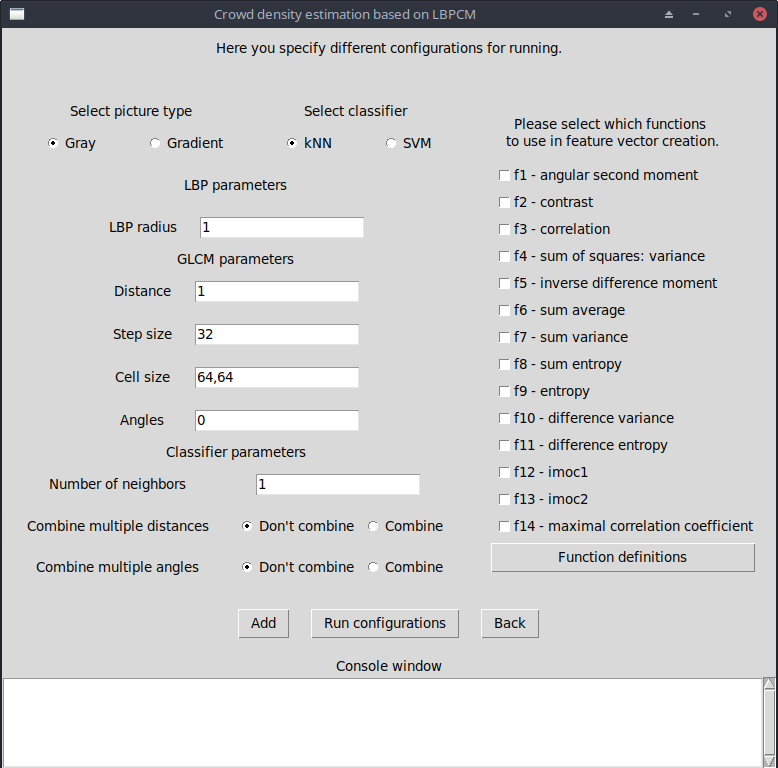
\includegraphics[scale=0.35]{img/fvc2.png}
\captionof{figure}{Izgled prozora za stvaranje konfiguracije}
\end{minipage}

\bigbreak

Prozor za stvaranje konfiguracije sastoji se od lijevog i desnog dijela. 
Lijevi dio služi za unos parametara dok je u desnom dijelu moguće odabrati
Haralickove značajke koje se izračunavaju iz LBPCM. Na vrhu prozora potrebno
je odabrati vrstu slike nad kojom se primjenjuje LBP operator: sliku 
sivih razina (\textit{gray}) ili sliku sivih razina nad kojom je 
primijenjen operator gradijenta (\textit{gradient}). 

\bigbreak

Za odabir klasifikatora postoje dvije mogućnosti: \textit{k}-NN klasifikator i 
SVM. Odabranom klasifikatoru se prosljeđuju stvoreni vektori značajki gdje se onda
interno spreme u slučaju \textit{k}-NN ili upotrijebe u fazi učenja klasifikatora
u slučaju SVM. 

\begin{table}
\begin{tabular}{p{0.35\linewidth} | p{0.6\linewidth}}
Parametar & Opis \\
\hline
LBP radius & označava veličinu radijusa oko središnjeg piksela
na temelju kojeg se izračunava LBP neke slike \\

\\
\hline
Distance & predstavlja udaljenost u LBPCM na temelju koje 
se gledaju pojavnosti sivih razina. Moguće je istovremeno izračunavati vrijednosti
za više udaljenosti, a u tom slučaju ih je potrebno odvojiti zarezom \\

\\
\hline
Step size & veličina koraka u x i y smjeru prilikom tehnike klizećeg okna \\

\\
\hline
Cell size & veličina putujućeg okna u smjeru x, y \\

\\
\hline
Angles & su svi kutovi za koje se konstruira LBPCM, odvajaju
se zarezom i upisuju u stupnjevima \\

\\
\hline
Number of neighbors & koristi se kod \textit{k}-NN klasifikatora
gdje označava broj susjeda na temelju čijeg se glasanja daje labela novome uzorku \\

\\
\hline
Combine multiple distances & predstavlja opciju kombiniranja više
udaljenosti u jednu, npr. ako je LBPCM izračunavana za udaljenosti 1, 2 i 3, matrice
se zbroje i podijele s 3 ako bi se odabrao slučaj s kombinacijom udaljenosti \enquote{combine}
u suprotnom se svaka interpretira za sebe \\

\\
\hline
Combine multiple angles & jednako kao i za udaljenosti

\end{tabular}
\caption{Opis parametara konfiguracije}
\end{table}

\bigbreak

Desna strana prozora prikazuje svih 14 Haralickovih značajki. Jednom kada 
su odabrani svi parametri s lijeve strane, desna strana se koristi za odabir 
značajki koje se izračunavaju prilikom kreiranja vektora značajki svake pojedine
konfiguracije. Svaka konfiguracija može imati broj značajki veći ili jednak jedan. 
Ovisno o broju odabranih značajki i broju različitih udaljenosti i kutova, vrijeme
stvaranja vektora značajki može biti značajno dugačko stoga se u fazi eksperimentiranja
stvara više konfiguracija koje se mogu izvoditi istovremeno ukoliko je računalo
višeprocesorsko. Definicije Haralickovih značajki moguće je vidjeti u dodatku A
ili pritiskom na gumb \enquote{Function definitions} nakon čega se otvara novi
prozor u kojem je naveden algebarski oblik svake Haralickove značajke kao i 
opisi drugih oznaka korištenih u formulama. 

\bigbreak

Nakon odabira željenih Haralickovih
značajki moguće je pritisnuti na gumb \enquote{Add} čime se stvara
nova konfiguracija. Ukoliko želimo dodati još konfiguracija, potrebno je samo
označiti ili izmijeniti postojeće parametre i opet pritisnuti gumb \enquote{Add}.
Svakim pritiskom gumba stvara se nova konfiguracija i interno pohranjuje te čeka na
pokretanje postupka stvaranja vektora značajki. Kada smo dodali sve konfiguracije
koje želimo, za početak stvaranje vektora značajki potrebno je pritisnuti gumb
\enquote{Run configurations} čime se onoliko konfiguracije izvodi paralelno koliko
naše računalo raspoloživih procesora ima. 

\bigbreak

Za praćenje napretka pokrenutih konfiguracija može se pritisnuti gumb 
\enquote{Back} koji otvara prethodnu stranicu sa slike 4.7 samo što su sada
u središnjem dijelu stranice trake napretka svake od dodanih konfiguracije od maloprije. 
Kraj svake konfiguracije je brojač koji prati broj do sada obrađenih, odnosno
stvorenih vektora značajki. Stranica s konfiguracijama prikazana je na slici 4.9, a 
napreduju samo dvije konfiguracije jer trenutno računalo ima samo dva raspoloživa procesora.
Po završetku jedne od prve dvije se pokreće treća i tako sve do završetka svih 
dodanih konfiguracija. Nakon završetka svake konfiguracije objekt koji predstavlja 
model klasifikatora sprema se na disk kako i konfiguracija samog modela kako
bi se kasnije prilikom faze klasifikacije mogao učitati ispravan model.

\bigbreak

\begin{minipage}{\linewidth}
\centering
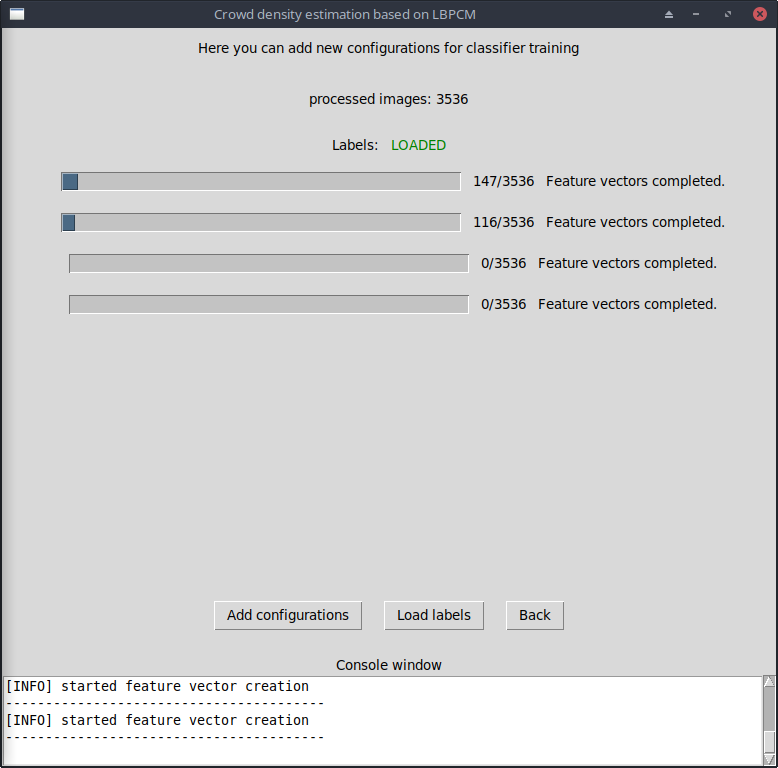
\includegraphics[scale=0.4]{img/fvc3.png}
\captionof{figure}{Prikaz napretka pojedinih konfiguracija}
\end{minipage}

\subsection{Klasifikacija slike postojećim modelima}

Jednom kada je stvaranje vektora značajki završeno i kada je model spremljen 
moguće je pristupiti postupku klasifikacije dosad neviđene slike. Kako bi se pristupilo 
stranici za klasifikaciju potrebno je 
pritisnuti gumb \enquote{Classification} koji se nalazi na glavnoj 
stranici aplikacije. Izgled stranice za klasifikaciju prikazan je na 
slici 4.10.

\bigbreak 

Na stranici je prikazana konfiguracija nekog modela koji se nalazi na 
disku računala. Prikazane su sve komponente konkretne konfiguracije
trenutnog modela, a uz to je i prikazana greška klasifikacije pod
nazivom \enquote{error}. Ta greška je omjer točno klasificiranih
podslika i ukupnog broja podslika koji se koristi za testiranje klasifikatora,
odnosno podslike koje nije vidio tijekom faze učenja. Ukoliko nije niti 
jedan model klasifikatora dostupan, prikazana je labela \enquote{NO MODEL}
koja javlja korisniku kako nije moguće klasificirati slike pošto nikakvog modela
nema.

\bigbreak

Trenutno je prikazan model koji je učen na slikama sivih razina i moguće
je vidjeti da trenutno takvih modela na disku ima 4 (redni broj modela
\enquote{Current model}). Kako bi vidjeli moguće modele koji su učeni na
gradijentnim slikama potrebno je pritisnuti gumb \enquote{Grad}.

\bigbreak

Za dohvat sljedećeg ili prethodnog dostupnog modela potrebno je pritisnuti na 
gumbe \enquote{Next} ili \enquote{Previous}. Jednom kada je odabran željeni
model za klasifikaciju potrebno je pritisnuti gumb \enquote{Load model} čime
se prikazani model učitava u memoriju i moguće ga je koristiti za klasifikaciju.
Ako je model ispravno učitan, tekst ispod trenutnog modela se mijenja
u \enquote{model loaded} sa zalenom kvačicom.

\bigbreak 

\begin{minipage}{\linewidth}
\centering
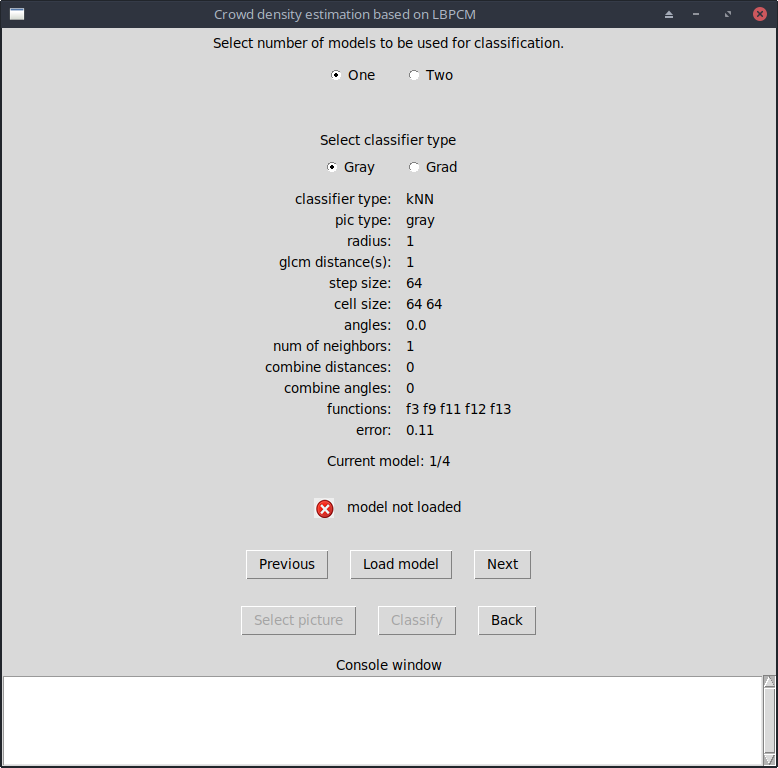
\includegraphics[scale=0.4]{img/cl1.png}
\captionof{figure}{Prikaz stranice za odabir jednog modela}
\end{minipage}

\bigbreak

Opisani postupak se primjenjuje kada želimo klasificirati novu sliku
koristeći samo jedan model. U slušaju da želimo koristiti kombinaciju
dva modela potrebno je pritisnuti gumb \enquote{Two} na vrhu stranice.
Nakon pritiska na gumb i učitavanja oba modela izgled stranice je prikazan
na slici 4.11. Jednom učitane modele moguće je koristiti za klasifikaciju. Kako
bi se odabrala željena slika za klasifikaciju potrebno je pritisnuti 
gumb \enquote{Select picture} nakon čega se otvara prozor za odabir slike.
Ako slika nije učitana, korisniku se ispisuje prikladna poruka te nije moguće 
nastaviti na klasifikaciju sve do kada se ne učita neka slika.
Nakon jednom učitane slike potrebno je pritisnuti na gumb \enquote{Classify} koji 
otvara prozor prikazan na slici 4.12.

\bigbreak 

\begin{minipage}{\linewidth}
\centering
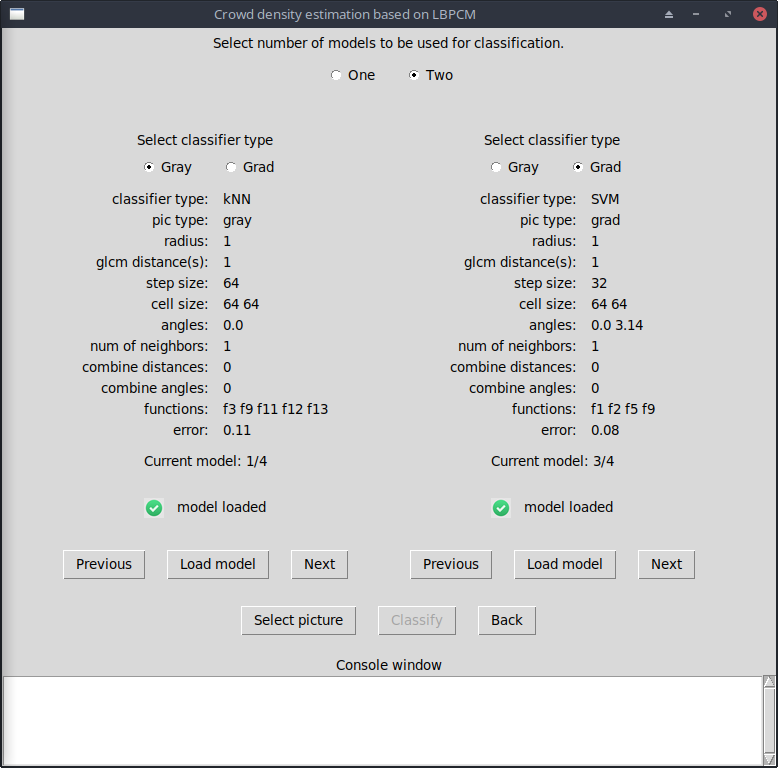
\includegraphics[scale=0.4]{img/cl2.png}
\captionof{figure}{Prikaz stranice za odabir dva modela}
\end{minipage}

\bigbreak

Na slici 4.12. prikazane su 3 identične kopije odabrane slike sljedećeg 
značenja. Na mjestu najveće slike će se prikazati rezultat klasifikacije kombinacije 
obaju modela dok su slike s desne strane rezultati klasifikacije svakog 
pojedinog klasifikatora. 
Razlog za to je uvid u utjecaj pojedinih težina svakog klasifikatora na 
krajnji rezultat klasifikacije. Vrh stranice prikazuje paletu boja koje
su dodijeljene pojedinom razredu gustoće mnoštva radi vizualnog
prikaza rezultata klasifikacije. Klasifikacija se napokon može pokrenuti
pritiskom na gumb \enquote{Start classification} nakon čega je potrebno
pričekati neko vrijeme koje ovisi o složenosti učitanog modela. 
Ovdje je moguće zamijetiti koliki utjecaj imaju različiti parametri i broj parametara 
na performanse programa i koje značajke se \enquote{isplati}
koristiti za stvaranje vektora značajki. Neke od značajki su izuzetno 
skupe za izračunavati i njihov doprinos možda i nije znatan u odnosu 
ne naku drugu koja se brže izračunava stoga je potrebno naći nekakav
kompromis između procesorskog vremena i točnosti klasifikatora jer 
nikome nije u cilju čekati neko duže vrijeme na rezultat klasifikacije pogotovo
ukoliko se radi o nekakvoj video sekvenci.
Podno najveće slike se nakon gotove klasifikacije prikazuje interval
procjene broja ljudi. Ako nije potrebno vidjeti rezultate svakog od
klasifikatora moguće je označiti  \enquote{Only voting classifier}
čime se samo klasificira najveća slika. Jednom kada je klasifikacija 
završila moguće je vidjeti rezultat na slici 4.13.

\bigbreak

\begin{minipage}{\linewidth}
\centering
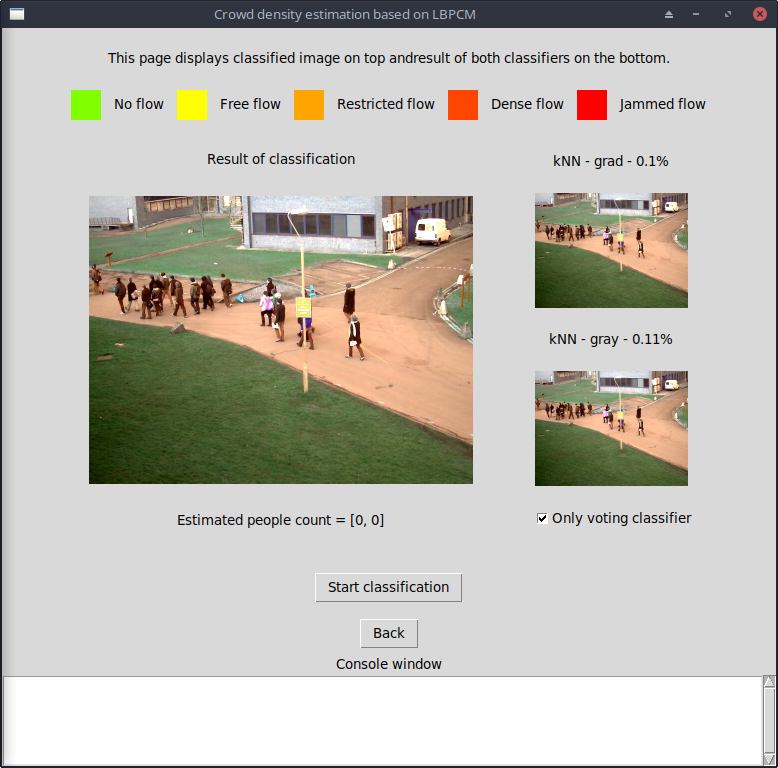
\includegraphics[scale=0.38]{img/cl3.png}
\captionof{figure}{Prikaz stranice za klasifikaciju slika}
\end{minipage}

\bigbreak

\begin{minipage}{\linewidth}
\centering
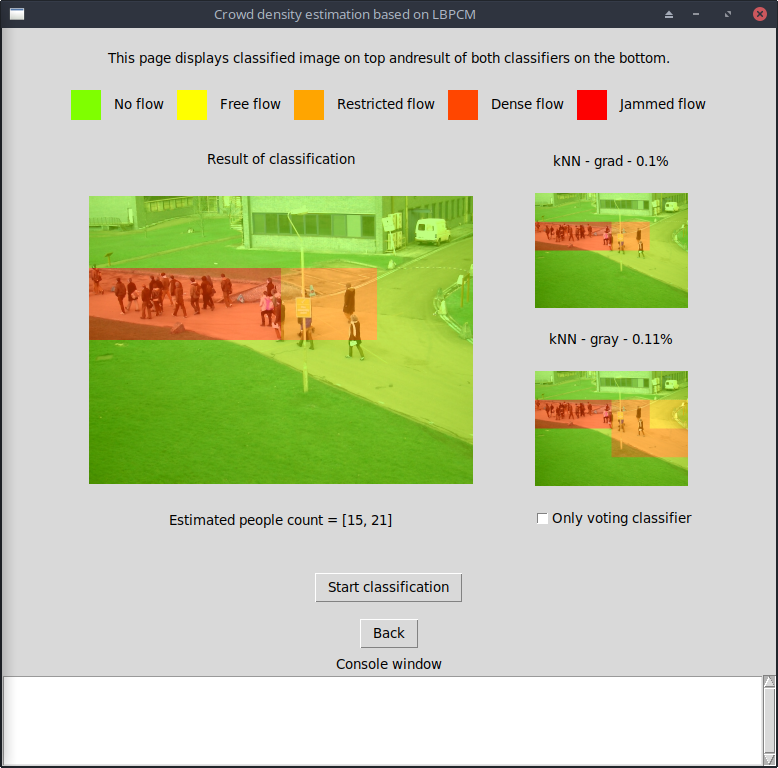
\includegraphics[scale=0.38]{img/cl5.png}
\captionof{figure}{Prikaz klasificirane slike i procjene broja ljudi na 
temelju gustoće mnoštva}
\end{minipage}

\newpage

Na slikama koje pokazuju rezultate klasifikacije pojedinih klasifikatora s 
desne strane može se zamijetiti kako točnosti klasifikacije utječu na
krajnji rezultat. Klasifikatori iz primjera nisu najbolje točnosti, 
međutim kada su upareni zajedno, mogu dati bolje rezultate kako je 
i ilustrirano na slici 4.13. To je i cijela ideja korištenja skupnog
klasifikatora koji spaja više njih u jednu cjelinu, u ovom slučaju
dva. 

\bigbreak

Iako se čini iz navedenog primjera da je rezultat samo preslika 
klasifikatora koji ima veću točnost klasifikacije, to ne mora uvijek 
biti slučaj. Nekad može fokus jednog klasifikator biti usmjeren 
na određene dijelove slike koji je možda uvjetovan odabranim 
Haralickovim značajkama, uvjetima osvjetljenja, kutom nagiba kamere ili 
nečim drugim dok drugi klasifikator može imati fokus na sasvim drugi 
dio slike. 

\bigbreak

Opisani problem bi se manifestirao na način da su neka 
područja slike, koja su u fokusu klasifikatora, ispravno klasificirana 
dok druga nisu te jednako tako i za drugi klasifikator, ali kada
su \enquote{spojeni} zajedno, daju jedan rezultat koji može biti bolji od 
svakog pojedinog klasifikatora. Pozitivne strane jednog klasifikatora mogu nadjačati 
negativne strane drugog klasifikatora i na kraju rezultirati uspješnom
procjenom gustoće mnoštva. Ta fuzija klasifikatora uvelike je određena 
težinama koje množe pojedine vjerojatnosne vrijednosti svakog klasifikatora.


\chapter{Tehnika klizećeg okna}

Kao jednu od osnovnih alatki postupka prikazanog u ovom radu, tehniku
kliznog okna moguće je vidjeti pritiskom na gumb \enquote{Sliding window}
na glavnoj stranici aplikacije. 

\bigbreak

\begin{minipage}{\linewidth}
\centering
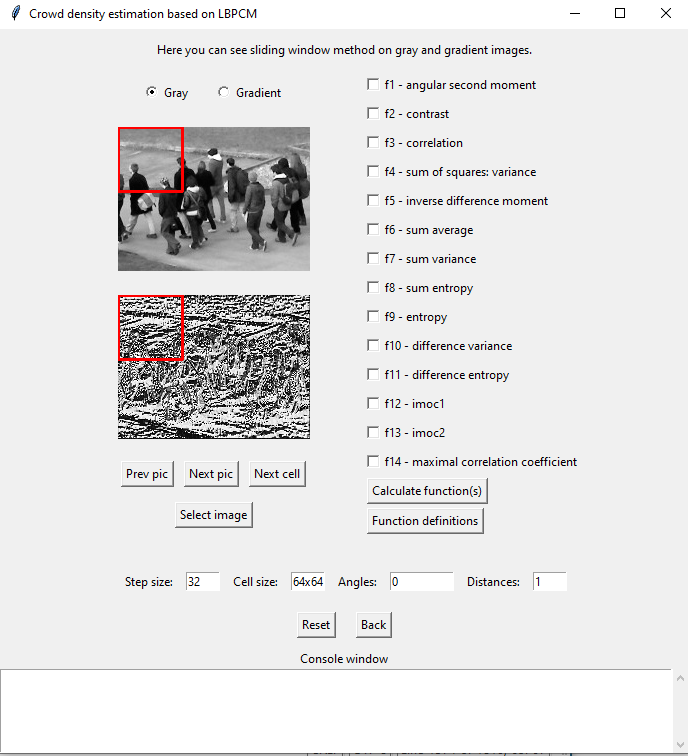
\includegraphics[scale=0.6]{img/sw1.png}
\captionof{figure}{Prikaz prozora tehnike klizećeg okna}
\end{minipage}

\bigbreak

Na slici 5.1 prikazane s dvije podslike koje su izravno učitane iz direktorija
s već obrađenim podslikama za ilustraciju postupka. Ukoliko je prikazan tekst 
\enquote{NO IMAGE} na mjestu namijenjenom za slike, to znači da još nisu 
izvorne slike obrađene i da podslike 
još ne postoje pa je potrebno učitati sliku iz nekog drugog direktorija pritiskom 
na gumb \enquote{Select Image} nakon čega se otvara prozor za odabir željene podslike.

\newpage

Na vrhu prozora postoje mogućnosti prikaza postupka nad podslikama sivih
razina i nad slikama koje su također sive razina, ali se nad njima još dodatno 
primijeni operator gradijenta. Za promjenu iz jednog stanja u
drugo potrebno je samo pritisnuti na željeni gumb. Za pomicanje okna na sljedeću
poziciju zaslužan je gumb \enquote{Next cell}. Pritiskom na dotični gumb se okno, koje
je na slici prikazano crvenim rubovima, pomiče na sljedeću poziciju. Sljedeća slika iz 
direktorija obrađenih podslika dohvaća se pritiskom na gumb \enquote{Next pic}, a 
prethodna gumbom \enquote{Prev pic}. Podnožje prozora zaokupljaju 
područja za upis parametara vezanih uz LBP i LBPCM. Pretpostavljene vrijednosti
su prikazane ulaskom u prozor i ukoliko se želi vidjeti utjecaj drugačijih parametara,
potrebno je upisati novu vrijednost parametra u odgovarajuće područje za upis i
pritisnuti na gumb \enquote{Reset} čime se ažurira podslika i resetira pozicija 
klizećeg okna.

\bigbreak

Želimo li izračunati vrijednosti konkretnih Haralickovih značajki 
trenutnog okna potrebno je odabrati sve željene značajke u desnom dijelu
prozora te pritisnuti gumb \enquote{Calculate funciton(s)}. Ukoliko
nije jasno kako su neke značajke definirane, moguće je vidjeti njihov
algebarski zapis pritiskom na gumb \enquote{Function definitions}. 
Nakon pritiska na gumb za izračun Haralickovih značajki, njihove vrijednosti
se pojavljuju u konzoli aplikacije. Izračun Haralickovih značajki se ovdje 
ne izračunava svakim pomakom okna jer su neke značajke iznimno 
računski zahtjevne, a i možda nam neka područja podslike nisu zanimljiva
pa se značajke samo izračunavaju pritiskom na odgovarajući gumb.

\bigbreak

Pogledom u izračune različitih Haralickovih značajki može se zamijetiti da vrijednosti funkcija 
odskaču u nekoliko redova veličina jedne od drugih, stoga ih je potrebno normalizirati
prije nego što se vektori značajki predaju klasifikatoru. Normalizacija
je nužan postupak iz razloga što ovdje korišteni klasifikatori koriste mjeru udaljenosti
kao funkciju koja određuje pripadnost nekom razredu te ako bi ostavili 
vrijednosti ovakvima, neke od njih uopće ne bi imale ikakvog utjecaja zbog 
svoje veličine dok bi druge, koje su možda manje važne u nekim slučajevima,
dominirale i previše utjecale na krajnji rezultat klasifikacije. Postoje više različitih 
metoda kojom se vektori značajki normaliziraju, npr. min-max, oko srednje vrijednosti, 
normalizacija z-ocjenom, skaliranje na jedinični vektor i dr. 

\bigbreak

U ovom radu je odabrana normalizacije kojom se vektori značajki svode na srednju vrijednost oko 0
i jediničnu varijancu.

\newpage

Postupak normalizacije:
\begin{center}

N - ukupan broj vektora značajki, \(k\) - k-ta komponenta vektora značajki

\begin{enumerate}
\item Izračun srednje vrijednosti svake komponente vektora značajki
\[
x_k = \frac{1}{N}\sum_{i=1}^{N}x_{ik}
\]

\item Izračun standardne devijacije svake komponente vektora značajki
\[
\sigma_k^2 = \frac{1}{N-1}\sum_{i=1}^N\left(x_{ik}-x_k\right)^2
\]

\item Od vrijednosti svake komponente vektora značajki se oduzme srednja
vrijednost te koponente i podijeli drugim korijenom iz srednje vrijednosti
devijacije te komponente

\[
x_{ik} = \frac{x_{ik}}{\sigma_k}
\]

\end{enumerate}
\end{center}

Nakon postupka normalizacije svi vektori imaju srednje vrijednosti oko nule
i jediničnu varijancu. 

\bigbreak
\underline{\textbf{Primjer} - Stvaranje vektora značajki}
\bigbreak

Kao primjer uzmimo 4 Haralickove značajke: kontrast, energiju, homogenost i entropiju. 

\bigbreak

Uvedimo oznake radi jednostavnijeg prikaza: 
\newline \(X_i,j\) predstavlja vrijednost funkcije kontrasta za \(i\)-ti
kut i \(j\)-tu udaljenost u GLCM
\newline \(Y_{i,j}\) predstavlja vrijednost funkcije energije za \(i\)-ti
kut i \(j\)-tu udaljenost u GLCM
\newline \(Z_{i,j}\) predstavlja vrijednost funkcije homogenosti za \(i\)-ti
kut i \(j\)-tu udaljenost u GLCM
\newline \(W_{i,j}\) predstavlja vrijednost funkcije entropije za \(i\)-ti
kut i \(j\)-tu udaljenost u GLCM

\bigbreak

Ukoliko bi uzeli udaljenost \(d=1\) i kutove \(\frac{\pi}{4}, \frac{\pi}{2}, \pi\)
kao parametre GLCM, vektor značajki jednog okna bi izgledao na sljedeći način:
\bigbreak
Radi jednostavnosti zapisa uvedimo indeks 1 za kut \(\frac{\pi}{4}\), 2 za
\(\frac{\pi}{2}\) i 3 za \(\pi\).

\bigbreak

\(
c = \left(X_{1,1}, X_{2,1}, X_{3,1}, Y_{1,1}, Y_{2,1}, Y_{3,1}, Z_{1,1}, 
Z_{2,1}, Z_{3,1}, W_{1,1}, W_{2,1}, W_{3,1}\right)
\)

\bigbreak

Kada je dobiven vektor značajki jednog okna, taj se vektor doda već postojećem 
vektoru značajki podslike te se postupak ponavalja za svako okno podslike.
\newline
Dimenzionalnost vektora značajki pojedinog okna dobije se umnoškom:

\begin{center}

\(A\) - broj Haralickovih značajki

\(B\) - broj kutova u GLCM

\(C\) - broj različitih udaljenosti u GLCM

\end{center}
\[
n = A \cdot B \cdot C = 4 \cdot 3 \cdot 1 = 12
\]

Broj okna u svakoj podslici može se izračunati prema formuli:

\begin{center}

\(X\) - širina podslike u pikselima
\(Y\) - visina podslike u pikselima
\(d_1\) - širina okna u pikselima
\(d_2\) - visina okna u pikselima
\(t\) - korak okna

\[
N = \left(\left\lfloor\frac{X-d_1}{t}\right\rfloor + 1\right) \cdot
\left(\left\lfloor\frac{Y-d_2}{t}\right\rfloor + 1\right)
\]

Ukupna dimenzionalnost vektora značajki pojedine podslike dobije se umnoškom:

\[
dim = N \cdot n
\]

Za konkretan slučaj s parametrima sa slike 5.1 i korištenim Haralickovim 
značajkama iz primjera iznad, dimenzionalnost vektora značajki bi iznosila:

\[
dim = 15 \cdot 12 = 180
\]

\end{center}

Iz primjera je vidljivo kako dimenzionalnost pojedine podslike može postati
iznimno velika. Izbor broja Haralickovih značajki, udaljenosti i broja kutova u 
LBPCM ima velik utjecaj na krajnju dimenzionalnost vektora značajki stoga je
od velike važnosti promišljanje o izboru parametara svakog modela. 


\chapter{Rezultati eksperimenta}

U svrhu boljeg razumijevanja dobivenih rezultata eksperimenta napravljena je manja  analiza
prostorne raspodjele uzoraka za svaki od razreda gustoće. Za analizu su uzeti sljedeći parametri:

\begin{table}[ht]
\centering
\begin{tabular}{c|c}
parametar & vrijednost \\
\hline
vrsta klasifikatora & \textit{k}-NN \\
broj susjeda & 1 \\
vrsta slike & sivih razina \\
LBP radijus & 1 \\
korak okna & 32 \\
veličina okna & 64x64 \\
LBPCM udaljenosti & 1 \\
LBPCM kutovi & 0, \(\pi\) \\
\end{tabular}
\caption{Prametri primjera} 
\end{table}

Analiza se također vrši nad skupom slika koji je korišten u radu. Stvoreni su vektori
značajki svake podslike, koji s navedenim parametrima poprimaju dimenzionalnost 240, 
normlizirani i raspoređeni na način da je svaki
od vektora značajki zbrojen zajedno s vektorima razreda kojem pripadaju.
Sljedeće su ti vektori uprosječeni čime je dobiven vektor značajki 
koji ne pripada niti jednoj podslici, a označava zamišljeno središte
pojedinog razreda (prototip), u fizici bi to bilo težište. 

\bigbreak

Nakon dobivenih središta razreda izračunate su euklidske udaljenosti između svakog
od razreda kako bi se dobila neka predodžba o razdiobi uzoraka u prostoru. 
Oznake u tablici 6.2 predstavaljaju razrede gustoće:\( c_0 \rightarrow \) \enquote{no flow},
\( c_1 \rightarrow \) \enquote{free flow}, \( c_2 \rightarrow \) \enquote{restricted flow}, 
\( c_3 \rightarrow \) \enquote{dense flow}, \( c_4 \rightarrow \) \enquote{jammed flow}.

Euklidska udaljenost se računa prema:
\[
d(x_1, x_2) = \sqrt{\left(\sum_{i=1}^{240} \left(x_{1i}-x_{2i}\right)^2\right)}
\]

\begin{table}[ht]
\centering
\begin{tabular}{c|c}
udaljenost između & iznos udaljenosti \\
\hline
\(d(c_0, c_1)\) & 4.49 \\
\(d(c_0, c_2)\) & 6.75 \\
\(d(c_0, c_3)\) & 10.11 \\
\(d(c_0, c_4)\) & 13.62 \\
\(d(c_1, c_2)\) & 4.69 \\
\(d(c_1, c_3)\) & 8.65 \\
\(d(c_1, c_4)\) & 12.5 \\
\(d(c_2, c_3)\) & 5.63 \\
\(d(c_2, c_4)\) & 9.98 \\
\(d(c_3, c_4)\) & 6.27
\end{tabular}
\caption{Euklidske udaljenosti među razredima} 
\end{table}

Iz priložene tablice moguće je vidjeti kako su središta razreda gustoća koji su bliski jedni drugima, npr.
\enquote{restricted flow} i \enquote{dense flow}, odnosno \(c_2\) i \(c_3\), bliža 
nego razreda koji su veoma različiti poput \(c_0\) i \(c_4\). Manja udaljenost središta znači
i povećana vjerojatnost krive klasifikacije. U idealnom slučaju bi razredi bili strogo odvojivi
i svaki razredi bi sačinjavali vektori značajki koji formiraju nekakav oblik hiperkugle ili nekog srodnog oblika
te ne bi postojali slučajevi gdje neke jedinke previše odskaču od središta svoga razreda i oblika toga razreda.
Stvarni život nije savršen te postoji skoro uvijek neki primjer koji je poseban.  Potrebno je naglasiti da
su udaljenosti izračunate nad normaliziranim vektorima pa su radi toga razloga toliko male.

\bigbreak

U te posebne slučajeve
spadaju pogreške prilikom označavanja uzoraka i uzorci koje je moguće svrstati u više različitih razreda. Primjer je
segmentacija izvorne slike u manje podslike gdje se stvara podslika koja cijepa gusto mnoštvo na dva dijela
i sad je problematično jer klasifikator ne zna da li gleda samo gustoću mnoštva koje je prepolovljeno ili gustoću 
tog mnoštva naspram površine cijele podslike čime dolazi u konflikt jer se dvoumi između dva različita razreda gustoće.
Isto tako, baš kao i klasifikator, čovjek se nekad može dvoumiti prilikom označavanja uzoraka
odgovarajućim razredima gustoće. Iz istih razloga naša odluka jednom može biti u jednom smjeru, a 
drugi put u drugom smjeru čime unosimo nekonzistentnost u skup podataka za učenje. Izbjegavati takve
stvari nije lako te je zbog toga potrebno imati čim veći skup podataka kako bi se posebni slučajevi
dovoljno malo puta pojavili i kako ne bi stvarali prevelikog utjecaja na ostatak skupa. 


\begin{table}[ht]
\parbox{.45\linewidth}{
\centering
\begin{tabular}{c|c}
udaljenost između & iznos udaljenosti \\
\hline
\(d(x_0, c_0)\) & 10.03 \\
\(d(x_0, c_1)\) & 10.91 \\
\(d(x_0, c_2)\) & 10.63 \\
\(d(x_0, c_3)\) & 12.74 \\
\(d(x_0, c_4)\) & 13.08 \\
\end{tabular}
\caption{Uzorak koji pripada razredu \enquote{no flow}}
}
\hfill
\parbox{.45\linewidth}{
\centering
\begin{tabular}{c|c}
udaljenost između & iznos udaljenosti \\
\hline
\(d(x_1, c_0)\) & 11.4 \\
\(d(x_1, c_1)\) & 10.93 \\
\(d(x_1, c_2)\) & 10.33 \\
\(d(x_1, c_3)\) & 11.75 \\
\(d(x_1, c_4)\) & 13.37 \\
\end{tabular}
\caption{Uzorak koji pripada razredu \enquote{free flow}}
}
\end{table}
\vspace{-1.5em}
\begin{table}[ht]
\parbox{.45\linewidth}{
\centering
\begin{tabular}{c|c}
udaljenost između & iznos udaljenosti \\
\hline
\(d(x_2, c_0)\) & 21.46 \\
\(d(x_2, c_1)\) & 20.33 \\
\(d(x_2, c_2)\) & 19.75 \\
\(d(x_2, c_3)\) & 17.86 \\
\(d(x_2, c_4)\) & 19.38 \\
\end{tabular}
\caption{Uzorak koji pripada razredu \enquote{restricted flow}}
}
\hfill
\parbox{.45\linewidth}{
\centering
\begin{tabular}{c|c}
udaljenost između & iznos udaljenosti \\
\hline
\(d(x_3, c_0)\) & 23.25 \\
\(d(x_3, c_1)\) & 22.55 \\
\(d(x_3, c_2)\) & 21.33 \\
\(d(x_3, c_3)\) & 18.26 \\
\(d(x_3, c_4)\) & 18.37 \\
\end{tabular}
\caption{Uzorak koji pripada razredu \enquote{dense flow}}
}
\end{table}


\vspace{-1.5em}
\begin{table}[!ht]
\parbox{.45\linewidth}{
\centering
\begin{tabular}{c|c}
udaljenost između & iznos udaljenosti \\
\hline
\(d(x_4, c_0)\) & 13.83 \\
\(d(x_4, c_1)\) & 13.35 \\
\(d(x_4, c_2)\) & 12.01 \\
\(d(x_4, c_3)\) & 9.37 \\
\(d(x_4, c_4)\) & 8.6 \\
\end{tabular}
\caption{Uzorak koji pripada razredu \enquote{jammed flow}}
}
\hfill
\parbox{.45\linewidth}{
\centering
\begin{tabular}{c|c}
ispravna oznaka & odluka klasifikatora \\
\hline
0 & 0 \\
1 & 1 \\
2 & 2 \\
3 & 3 \\
4 & 4 \\
\end{tabular}
\caption{Predočeni uzorci klasifikatoru i rezultati klasifikacije}
}
\end{table}

Za svaki od razreda uzet je jedan još neviđeni uzorak, izračunat je vektor značajki te je  za taj vektor
 izračunata udaljenost do svakog od središta razreda (\(c_o, c_1, c_2, c_3, c_4\)). Uz to je pripremljen 
\textit{k}-NN klasifikator s parametrima navedenim u tablici 6.1. Svaki od još neviđenih vektora
predat je klasifikatoru kako bi vidjeli i njegov odluku. Svaki \(x_i\) u tablicama iznad, gdje je \(i=0,1,2,3,4\),
označava pripadnika jednog od razreda gustoće.

\bigbreak

Iz tablice 6.8 moguće je vidjeti kako je klasifikator ispravno dodijelio oznaku svakome uzorku iako
je njegova točnost 90.52\%. Iščitavanjem tablica 6.3 - 6.7 zamjećuje se da se odluka klasifikatora
razlikuje od odluke koja bi se donijela ako bi se promatrale najmanje udaljenosti do središta pojedinih 
razreda gustoće. Razlog za takvu odluku klasifikatora je zbog principa najbližih \textit{k} 
susjeda, u ovom primjeru najbližeg jednog susjeda. Rezultati klasifikacije odgovaraju
najbližim središtima za slučajeve razreda: 0, 3, 4 dok je kod ostalih središte razreda različito od
dodijeljene odluke. 

\bigbreak

Primjer pokazuje kako je veoma važno uzeti prikladnu mjeru udaljenosti koju klasifikator koristi
za usporedbu dva različita uzorka. Pritom nije svejedno uspoređuje li se nepoznati 
uzorak sa svim ostalim uzorcima ili samo onim umjetnim uzorcima koji bi trebali
predstavljati središta svakog od razreda. Izbor vrste usporedbe pojedinih vektora
značajki ovisi o samim podatcima koje koristimo za učenje klasifikatora. Ako su nepravilne
grupe vektora značajki u \textit{n}-dimenzionalnom prostoru, možda je bolja ideja izabrati
klasifikaciju prema biližim susjedima dok u slučaju da imamo donekle pravilne grupe (hiperkugle i sl.) 
je bolje izabrati središta pojedinih razreda kao vektore s kojima se svi dosad neviđeni uspoređuju
jer i time u krajnjem slučaju štedimo vrijeme potrošeno na usporedbu. 

\bigbreak

Eksperimentom se došlo do zaključka kako \textit{k}-NN klasifikator daje dobre rezultate
za manje vrijednosti broja \textit{k} pri čemu je on neparan i to za vrijednosti \(k=1\) ili \(k=3\).
Većim vrijednostima se unosi određena greška jer raspodjela vektora značajki nije uvelike pravilna.
Veličina koraka okna od 64 i 32 piksela pokazala se kao najbolja  mjera obzirom na veličinu okna od 64x64. 
Manji koraci ne donose nikakvu novu informaciju nego samo povečavaju vrijeme potrebno za 
obradu pojedine podslike, a koraci veći od 64 nemaju smisla obzirom da je veličina okna zadržana
stalnom. 

\bigbreak

Općenito je uvođenje većeg broja različitih vrijednosti kutova davalo bolje rezultate
vezano uz točnost klasifikacije međutim pogledom u tablicu rezultata u dodatku B moguće je 
vidjeti kako postoje modeli klasifikatora koji rade samo s kutem od 0 stupnjeva i postižu
bolje rezultate od nekih drugih koji imaju npr. 4 različita kuta. Klasifikatori koji su koristili
slike sivih razina generalno imaju neznatno veću točnost klasifikacije u usporedbi s klasifikatorima 
koji rade sa slikama sivih razina nad kojima je primijenjen operator gradijenta, pritom su obje vrste
klasifikatora imala iste parametre osim vrste slike koju koriste.

\bigbreak

Izbor Haralickovih značajki koje će model klasifikatora koristiti za izračunavanje nad nekom
podslikom je jedna od najvažnijih ako ne i najvažnija stavka. Važno je napomenuti kako se
pojedine značajke mogu izuzetno brzo izračunati jer je npr. potrebna samo suma LBPCM
pomnožena s nekim brojem dok druge značajke izuzetno vremenski opterete postupak 
učenja pa je stoga izbor značajki ogreničeni i tom ogradom. U ovom radu nikad nije uzeto
više od 7 različitih Haralickovih značajki zbog ograničenih računalnih i vremenskih resursa.
Smisleno je koristiti skup parametara koji nije prezahtjevan jer preveliko čekanje na klasifikaciju
slike nije poželjno u situacijama koje zahtijevaju možda brzu reakciju. Druga opcije je 
koristiti grafičke procesore i paralelizirati koliko je to moguće sam postupak izračunavanja
čime se automatski diže kompleksnost samog sustava.

\bigbreak

U radu \citep{6266412} odabrane su Haralickove značajke: energija, kontrast,
homogenost i entropija. Te konkretne značajke veoma se brzo daju izračunati, a daju 
vrlo dobre rezultate kako je vidljivo iz tablice u dodatku B. Izbor tih značajki uvelike poboljšava
performanse samog postupka naspram nekih drugih izbora parametara s više različitih značajki, a
ne narušava značajno točnost klasifikacije. Postoje bolji odabiri značajki, ali kako je već navedeno, 
računski su zahtjevniji i time njihovo korištenje baš nema smisla. 

\bigbreak

Pogledom u tablicu rezultata eksperimenta moguće je također vidjeti kako neke konfiguracije 
kreću s četiri različite Haralickove značajke i onda im se dodaje po jedna nova značajka ne bi
li se točnost povećala. U nekim slučajevima se dodavanjem novih značajki točnost čak i smanjila
što ukazuje na to da nije za povećanje točnosti samo dovoljno dodati veliki broj značajki nego 
treba dobro promisliti i eksperimentom pokušati doći do zaključka. Pokazalo se kako najbolji skup
značajki sadržava: entropiju, homogenost, kontrast i energija kako je i navedeno u radu Wanga i drugih.
Odabir ovih značajki je smislen jer pružaju veoma dobru točnost klasifikacije, a i 
vrijeme izračuna nije veliko. Kao dodatna mjeru robusnosti ima smisla koristiti takav klasifikatora na sivim
slikama u fuziji s drugim koji koristi gradijentne slike čime se točnost klasifikacije može podići
za nekoliko postotaka.


\chapter{Prikladnost korištenog postupka na drugome skupu podataka}

Postupak pripazan u ovome radu prikladan je za vrstu slika kojima se parametri ne mijenjaju. Pod 
pojmom parametri misli se na položaj ili kut kamere, osvjetljenje slike ili preveliku gustoću mnoštva, 
primjerice mnoštvo gledano iz zraka. Korištenjem lokalne binarne značajke i tehnike kliznog prozora
nije moguće izvući neko smisleno značenje iz sivih razina slike. Haralickove značajke imaju
mogućnost izvlačenja neke vrste informacija iz slike što na kraju rezultira određenom vrijednošću
koja odgovara pojedinome oknu. Za ograničen skup slika, vrijednosti Haralickovih značajki 
se kreću u nekom intervalu te se stoga predočavanjem nove, još dosad neviđene slike koja
svojim teksturnim sastavom ne odgovara dosad viđenim slikama, u klasifikatoru stvara pomutnja.
Takva slika može biti veoma udaljena od svakog središta razreda i najbližeg uzorka stoga 
će se s velikom vjerojatnošću krivo klasificirati. 

\bigbreak

Zbog navedenih razloga korištenje jednom već naučenog klasifikatora nad novim skupom
slika rezultira poražavajućom točnošću klasifikacije. Takvi rezultati mogu se izbjeći
ponovljenim postupkom prikazanim na slici 3.2 koji uključuje ponovnu podjelu
izvornih slika u manje podslike, ručno označavanje pojedinih razreda gustoće i 
na kraju stvaranje vektora značajki. 

\bigbreak

Iako ova metoda nije tolike općenitosti da bi jednom naučeni klasifikatori mogli
prepoznavati mnoštvo na bilo kakvim slikama, dovoljno je općenita i jednostavna
da se u primjenjuje u uvjetima gdje se parametri slike ne mijenjaju ili se mijenjaju vrlo
malo. Primjer takvih primjerna je identifikacija osobe temeljem otiska dlana \citep{1512051}
ili u trgovačkim centrima u kojima su uvjeti osvjetljenja i položaj kamere nepromijenjeni.

\bigbreak

Za ilustraciju navedenih tvrdnji uzet je jedan novi skup podataka, odnosno slika. Hrvatska 
nogometna reprezentacija je 2018. godine postigla izniman uspjeh, osvojivši drugo mjesto
na svjetskom prvenstvu. Povratak pripadnika nogometne reprezentacije (Vatrenih) snimljen
je od strane Hrvatske radiotelevizije te ga je moguće pogledati na stranicama youtube.com
servisa \citep{vatreni}. Upravo je uzet djelić snimke gdje su snimljene 
velike grupe ljudi u ukupnom trajanju od deset sekundi.  

\bigbreak

\begin{minipage}{\linewidth}
\centering
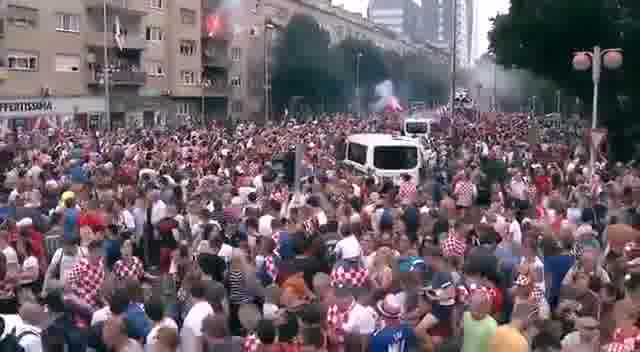
\includegraphics[scale=0.5]{img/data2.jpg}
\captionof{figure}{Prikaz jedne od slika novog skupa podataka}
\end{minipage}

\bigbreak

Na slici 7.1 vidljivo je koliko su dva korištena skupa podataka različita. Prvi skup sadrži
manje grupacije ljudi do tridesetak ljudi, dok se kod drugog skupa toliko ljudi može naći
samo u jednoj podslici. Iz priloženog se može zaključiti kako primjena jednog od naučenih klasifikatora
nije moguća na potpuno novom skupu podataka jer se mogu razlikovati u veličini slike, 
broju podslika, koraku i veličini okna te brojnim drugim parametrima. 

\bigbreak 

Kako nije moguću izravna primjena već naučenih klasifikatora, ponovljen je postupak 
prikazan na slici 3.2. Snimka Vatrenih je podijeljena na sličice kojih je ukupno ispalo 200. 
Rezolucija svake slike iznosi 640x352 piksela što je manje nego izvorni skup podataka 
nad kojim se prvotno vršilo eksperimentiranje. Kako bi se održvala neka vrsta usporedivosti,
 slike novog skupa također su podijeljene u 16 jednakih podslika, svaka dimenzija 160x88 piksela. 
Jednom podijeljene slike su ručno označene te je pokrenut postupak
stvaranja vektora značajki. Korišteni su drugačiji parametri nego dosad gdje je za
veličinu okna uzeto 40x40 piksela kako bi se pokrila cijela slika i korak okna od 20 piksela.
Odabrane Haralickove značajke su: energija, homogenost, homogenost i kontrast.

\bigbreak

Kako nije svrha tražiti optimalne parametre drugog skupa podataka nego samo pokazati 
korisnost postupka opisanog u radu, svega je par puta pokrenut postupak učenja nakon 

\begin{figure}[ht]
	\begin{subfigure}[b]{0.19\linewidth}
		\centering
		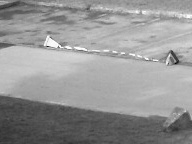
\includegraphics[scale=0.5]{img/noflow.jpg}
		\caption{No flow}
	\end{subfigure}
	\begin{subfigure}[b]{0.19\linewidth}
		\centering
		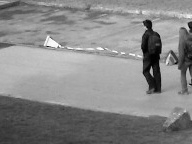
\includegraphics[scale=0.5]{img/freeflow.jpg}
		\caption{Free flow}
	\end{subfigure}
	\begin{subfigure}[b]{0.19\linewidth}
		\centering
		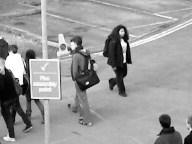
\includegraphics[scale=0.5]{img/restrictedflow.jpg}
		\caption{Restricted flow}
	\end{subfigure}
	\begin{subfigure}[b]{0.19\linewidth}
		\centering
		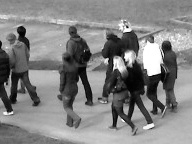
\includegraphics[scale=0.5]{img/denseflow.jpg}
		\caption{Dense flow}
	\end{subfigure}
	\begin{subfigure}[b]{0.19\linewidth}
		\centering
		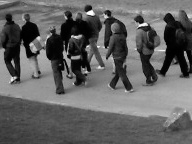
\includegraphics[scale=0.5]{img/jammedflow.jpg}
		\caption{Jammed flow}
	\end{subfigure}
\caption{Reprezentativni uzorci svakog od razreda prvog skupa podataka}
\end{figure}

\begin{figure}[ht]
	\begin{subfigure}[b]{0.19\linewidth}
		\centering
		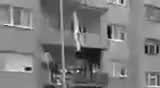
\includegraphics[scale=0.4]{img/noflow2.jpg}
		\caption{No flow}
	\end{subfigure}
	\begin{subfigure}[b]{0.19\linewidth}
		\centering
		
\includegraphics[scale=0.4]{img/freeflow2.jpg}
		\caption{Free flow}
	\end{subfigure}
	\begin{subfigure}[b]{0.19\linewidth}
		\centering
		
\includegraphics[scale=0.4]{img/restrictedflow2.jpg}
		\caption{Restricted flow}
	\end{subfigure}
	\begin{subfigure}[b]{0.19\linewidth}
		\centering
		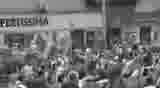
\includegraphics[scale=0.4]{img/denseflow2.jpg}
		\caption{Dense flow}
	\end{subfigure}
	\begin{subfigure}[b]{0.19\linewidth}
		\centering
		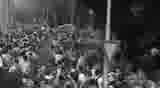
\includegraphics[scale=0.4]{img/jammedflow2.jpg}
		\caption{Jammed flow}
	\end{subfigure}
\caption{Reprezentativni uzorci svakog od razreda drugog skupa podataka}
\end{figure}

\bigbreak

kojeg je najbolji rezultat imao točnost od 77.79\%. Ovakva točnost klasifikatora nikako
nije idealna, a to može biti iz nekoliko razloga. Pogreške kod označavanja podslika je 
već naveden kao jedan od problema koji se može javiti, zatim nedovoljno ispitivanje
različitih vrijednosti parametara i Haralickovih značajki. Novi problem koji je utjecao
na točnost, a nije prisutan u prvom skupu podataka su nedovoljno jasne i čiste podslike.
Naime rezolucija izvornog videozapisa bila je 480p, što i nije toliko loše, međutim platforme 
poput youtube.com koriste različite algoritme kompresije kako bi se uštedjelo na mjestu i 
time povećao protok informacija. Navedene kompresije spadaju u vrstu kompresija s gubitcima, 
odnosno u pojedinim sličicama videozapisa počinju se javljati različiti fragmenti koji narušavaju 
ukupnu kvalitetu slike što na kraju rezultira

\bigbreak

\begin{minipage}{\linewidth}
\centering
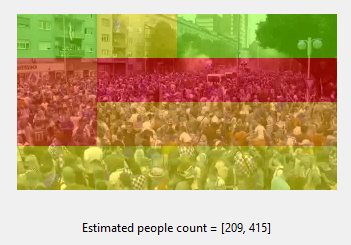
\includegraphics{img/clas2.png}
\captionof{figure}{Klasificirana slika novog skupa podataka}
\end{minipage}

\noindent uništenim detaljima koji su u ovom slučaju znatni jer su mnoštva velika, a veličina glave 
pojedinog čovjeka je mala. Kompresija jednog takvog videozapisa može rezultirati 
fragmentima jednake boje koji nadomještaju glave nekoliko
ljudi čime se gubi na informaciji koju je moguće izvući iz slike Haralickovim značajkama.

\bigbreak

Prikaz usporedbe dvaju skupova razreda prikazan je na slikama 7.2 i 7.3. Odmah je vidljivo 
koliko se izgled i gustoća mnoštva razlikuju. Slika 7.4 prikazuje rezultat klasifikacije jedne do sada
neviđene slike za klasifikator. Iako je točnost klasifikacije znatno manja od klasifikatora na prijašnjem
skupu podataka, mogu se lijepo vidjeti različiti slojevi gustoće mnoštva i rezultat na prikazanoj slici
je zadovoljavajuć osim što je veoma teško podesiti intervale ljudi koje pojedini razred gustoće 
predstavlja stoga intervali procjene ljudi mogu biti dosta široki. 

\bigbreak

Odabir ovdje navedenih parametara je bio brzinski i nije uložen prevelik trud u učenje novog 
klasifikatora, osim označavanja podslika, a dobiven je rezultat koji zadovoljava. Jednom razvijen
sustav kao u ovom radu sposoban je davati dobre rezultate nad različitim gustoćama mnoštva
ukoliko se postupak učenje ponovi prilikom promjene skupa podataka i ukoliko se mnoštvo te uvjeti
u kojima je kamera znatno ne mijenjaju. Ako bi se sustav naučio na slikama gdje je mnoštvo kao na
slici 7.1, a drugi dan bi se gužva raščistila te bi ulice bile prazne, rezultati klasifikacije bi bili poražavajući
jer bi se teksturna svojstva slike drastično promjenila.

\chapter{Zaključak}

Kako je navedeno u i uvodu, procjena gustoće mnoštva izuzetno je važna komponenta sustava
za nadziranje i upravljanje mnoštvom. Video prijenos sigurnosnih kamera prilikom znatnijih 
okupljanja ljudi može se obraditi na način da prikazuju korisne informacije poput procjene
broja ljudi u svakoj sličici prijenosa ili označena mjesta od interesa koja ukazuju na kakvu 
nepravilnost ili potencijalnu opasnost. Takva mjesta mogu biti gužve, iznenadne promjene
sastava mnoštva ili npr. mjesta koja zahtijevaju održavanje socijalne distance, a ona sama
je narušena prevelikim brojem ljudi. Korištenje takvih sustava uvelike olakšava posao ljudi
zaduženih za obavljanje tih zadaća, ali i uvodi jednu novu razinu trenutnog odziva na novonastalu 
situaciju gdje svaka sekunda može biti važna. 

\bigbreak

Razvijen je relativno jednostavan sustav za procjenu gustoće i broja ljudi koji se temelji na 
tehnici kliznog okna i lokalnoj binarnoj značajki. Kako bi se povećala robusnost cijelog sustava
klasifikacija se sastoji od sjedinjenja dvaju različitih klasifikatora: jednog koji koristi slike
sivih razina i drugog koji koristi također slike sivih razina, ali je nad njima primijenjen operator 
gradijenta. Takva kombinacija klasifikatora generalno daje bolje rezultate i ima mogućnost
ispraviti pogrešne klasifikacije pojedinog klasifikatora tako što se važnost svakog klasifikatora
regulira težinom koja odgovara točnosti klasifikacije dotičnog. Regulirati te težine se može i 
na druge načine, ali pritom treba pripaziti jer to uvelike može promijeniti odluke klasifikacije.

\bigbreak

Ovakva fuzija dvaju klasifikatora pokazala se dobrom što je i na kraju rezulziralo zadovoljavajućim
rezultatima. Primjena operatora LBP i tehnike klizećeg okna nad slikama s mnoštvom omogućilo je 
izvlačenje informacija o slici koje su zatim korištene za izračune Haralickovih značajki. Iako nije moguće 
izravno povezati neku značajku i njezino značenje u smislu argumentiranja vrijednosti funkcije
nad nekom slikom, moguće je doći do zaključka kako je npr. vrijednost entropije veća za kompleksnije slike.
Provođenjem eksperimenta s različitim parametrima zaključeno je kako porast broja različitih 
parametara, odnosno dodavanje novih Haralickovih značajki, ne mora nužno značiti da će točnost
klasifikacije porasti. Uvođenje kompleksnijeg skupa parametara ima za posljedicu duže izvođenje
postupka klasifikacije, a porast točnosti nije znatan da bi se opravdalo veće čekanje na klasifikaciju.

\bigbreak 

Opisani razlozi ne znače da nije poželjno povećavati broj značajki. Povećanje je opravdavajuće
ako se problem prilagodi na način da se izračuni značajki paraleliziraju što je više moguće. 
Paralelizacija problema imala bi i više nego značajno poboljšanje performansi samog postupka
izračuna Haralickovih značajki gdje bi se svaka značajka, svakog okna podslike, mogla izračunavati sama 
za sebe, istovremeno sa svim ostalim. Za takav postupak mogu se koristiti grafički procesori
koji imaju i više no dovoljno jezgara za takve izračune. Upotreba grafičkih kartica za ubrzanje
postupka moglo bi dovesti do primjene metode opisane u radu za procjenu gustoće mnoštva 
u realnom vremenu s nekim pristojnim brojem sličica u sekundi.

\bigbreak

Prikladnost korištenja LBP i tehnike kliznog okna pokazana je u ovom radu, međutim jednom
naučeni klasifikatori na jednom skupu slika nisu u mogućnosti preslikati svoje znanje
na novi skup slika koji se od prošlog može razlikovati po broju ljudi, odnosno gustoći,
uvjetima osvjetljenja ili kutu kamere. To je ograničenje ovakvog postupka jer on 
nema mogućnosti izvlačenja semantičkog značenja piksela koji su mu predočeni 
u obliku slike. Pikseli sivih razina  svojim vrijednostima doprinose vrijednostima Haralickovih 
značajki, ali promjena svjetlosnih uvjeta odmah rezultira različitim vrijednostima sivih
razina i cijeli postupak više nije primjenjiv nad novom vrstom slika. Kako bi koristili 
opisani postupak nad novim skupom slika, potrebno ih je opet podijeliti u podslike, 
ručno označiti i opet provesti postupak učenja te prilagoditi parametre pojedinog klasifikatora
jer možda jednak skup parametara ne radi najbolje za različite skupove slika. 
Smisleno korištenje ovakvog sustava je opisano u \citep{1512051} gdje
se prepoznaje identitet osobe na temelju otiska ruke. Ovdje su uvjeti u kojim se 
dohvaća slika dlana skoro identični u svako doba dana i stoga nema veće razlike
u sivim razinama čime se veoma lako primjenjuje i daje izuzetne rezultate.

\bibliography{literatura}
\bibliographystyle{fer}

\listoffigures
\listoftables

\begin{sazetak}
Procjena gustoće mnoštva od velike je važnosti u video nadzoru i upravljanju mnoštvom. Predložene
su različite metode za rješavanje ovog problema, međutim, većina ih procjenjuje gustoću mnoštva
cijele slike pritom ignorirajući lokalna mnoštva. U ovom radu primjenjuje se operator lokalnih binarnih
značajki nad sivim slikama i sivim slikama nad kojima je primjenjen operator gradijenta. Iz takvih slika
se pomoću matrice pojavnosti lokalnih binarnih značajki, postupkom klizećeg okna, izračunavaju
 Haralickove značajke koje tvore vektore značajki. Koriste se dvije vrste klasifikatora: \textit{k}-NN i SVM koji 
se na kraju spajaju u jedan klasifikator i utjecaj svakog klasifikatora uvjetovan je njegovom točnošću 
klasifikacije.

\kljucnerijeci{Lokalna binarna značajka, Matrica pojavnosti lokalnih binarnih uzoraka, Vektor značajki, \textit{k}-NN klasifikator,
SVM klasifikator, gustoća mnoštva}
\end{sazetak}

\engtitle{Crowd density estimation based on local binary pattern co-occurence matrix}
\begin{abstract}
Crowd density estimation is of great importance in video surveillance and in crowd management. 
Most of the existing methods estimate crowd density of a whole image while ignoring local density areas.
In this work local binary pattern is used on gray and gradient images. These pictures are used to 
extract Haralick features from local binary pattern co-occurence matrix, using sliding window
technique, which later form feature vectors. Two type of classifiers are used: \textit{k}-NN and SVM.
They are later fused together and the influence of each one is dependant on the classifier accuracy of 
training set of images.

\keywords{local binary pattern, gray level co-occurence matrix, feature vectors, \textit{k}-NN, SVM, crowd density}
\end{abstract}

\appendix

\chapter{Teksturne značajke}

Oznake korištene dalje u tekstu:
\bigbreak
\(N_g\) - broj sivih razina
\(p(i,j)\) - \((i,j)\)-ti element normalizirane matrice pojavnosti sivih razina
\bigbreak
\(p_x(i)\) - \(i\)-ti element u matrici marginalnih vjerojatnosti koja je dobivena 
zbrajanjem redaka = \(\sum_{j=1}^{N_g}p(i,j)\)
\bigbreak
\(p_y(j)\) - \(j\)-ti element u matrici marginalnih vjerojatnosti koja je dobivena 
zbrajanjem stupaca = \(\sum_{i=1}^{N_g}p(i,j)\)

\[
p_{x+y}(k)=\sum_{i=1}^{N_g} \sum_{j=1}^{N_g} p(i,j) \;\;\; k=2,3,...,2N_g, \; i+j=k
\]

\[
p_{x-y}(k)=\sum_{i=1}^{N_g} \sum_{j=1}^{N_g} p(i,j) \;\;\; k=0,1,...,N_g-1, \; \left|i-j\right|=k
\]

\[
\sum_i \; \textrm{predstavlja pokratu} \; \sum_{i=1}^{N_g} \; \textrm{,a} \;
\sum_{j} \; \textrm{predstavlja pokratu} \; \sum_{j=1}^{N_g}
\]

\newpage

1) Angular second moment:
\[
f_1 = \sum_{i}\sum_{j}p(i,j)^2
\]

2) Contrast:
\[
f_2 = \sum_{n=0}^{N_g-1}n^2 \left( \sum_{i=1}^{N_g}\sum_{j=1}^{N_g}p(i,j) \right), \left| i-j \right| = n
\]

3) Correlation:
\[
f_3 = \frac{\sum_i\sum_j\left(ij\right)p(i,j) - \mu_x\mu_y}{\sigma_x\sigma_y}
\]

4) Sum of squares: variance:
\[
f_4 = \sum_i\sum_j(i-\mu)^2p(i,j)
\]

5) Inverse difference moment:
\[
\sum_i\sum_j \frac{1}{1+(i-j)^2}p(i,j)
\]

6) Sum of average:
\[
f_6 = \sum_{i=2}^{2N_g}ip_{x+y}(i)
\]

7) Sum variance:
\[
f_7 = \sum_{i=2}^{2N_g}(i-f_8)^2p_{x+y}(i)
\]

8) Sum entropy:
\[
f_8 = -\sum_{i=2}^{2N_g}p_{x+y}(i)\log(p_{x+y}(i))
\]

9) Entropy:
\[
f_9 = -\sum_i\sum_j p(i,j)\log(p(i,j))
\]

10) Difference variance
\[
f_{10} = \textrm{variance of} \; p_{x-y}
\]

11) Difference entropy:
\[
f_{11} = -\sum_{i=0}^{N_g-1}p_{x-y}(i)\log(p_{x-y}(i)) 
\]

12), 13) Information measures of correlation
\[
f_{12} = \frac{HXY - HXY1}{max\{HX,HY\}}
\]
\[
f_{13} = \sqrt{(1-\exp{-2(HXY2 - HXY)}}
\]
\[
HX = -\sum_i\sum_j p(i,j)\log(p(i,j))
\]
\[
HXY1 = -\sum_i\sum_j p(i,j)\log(p_x(i)p_y(y))
\]
\[
HXY2 = -\sum_i\sum_j p_x(i)p_y(y) \log(p_x(i)p_y(y))
\]

14) Maximal correlation coefficient:
\[
f_{14} = \sqrt{Second \; largest \; eigenvalue \; of \; Q}
\]
\[
Q(i,j) = \sum_k \frac{p(i,k)p(j,k)}{p_x(i)p_y(k)}
\]

\chapter{Rezultati eksperimenta}


\begin{adjustwidth}{-30pt}{0pt}
\begin{tabular}{c|c|c|c|c|c|c|c|c|c|c}
\STAB{\rotatebox[origin=c]{90}{redni broj}} & 
\STAB{\rotatebox[origin=c]{90}{\;\;vrsta klasifikatora\;\;}} & 
\STAB{\rotatebox[origin=c]{90}{vrsta podslike}} & 
\STAB{\rotatebox[origin=c]{90}{radijus}} & 
\STAB{\rotatebox[origin=c]{90}{GLCM udaljenosti}} & 
\STAB{\rotatebox[origin=c]{90}{korak okna}} & 
\STAB{\rotatebox[origin=c]{90}{veličina okna}} & 
\STAB{\rotatebox[origin=c]{90}{kutovi}} & 
\STAB{\rotatebox[origin=c]{90}{broj susjeda }}& 
\STAB{\rotatebox[origin=c]{90}{značajke}} & 
\STAB{\rotatebox[origin=c]{90}{greška}} \\
\hline
1 & \textit{k}-NN & grad & 1 & 1 & 32 & 64x64 & 0,\(\pi\)& 1 & f1,f2,f5,f9 & 9.9\% \\
2 & SVM & gray & 1 & 1 & 32 & 64x64 & 0,\(\pi\)& - & f1,f2,f5,f9 & 8.86\% \\
3 & SVM & grad & 1 & 1 & 32 & 64x64 & 0,\(\pi\)& - & f1,f2,f5,f9 & 7.92\% \\
4 & \textit{k}-NN & gray & 1 & 1 & 32 & 64x64 & 0,\(\pi\)& 1 & f1,f2,f5,f9 & 9.52\% \\
5 & SVM & gray & 1 & 1 & 32 & 64x64 & 0,\(\pi\)& - & f1,f2,f3,f4,f5,f9 & 8.39\% \\
6 & SVM & grad & 1 & 1 & 32 & 64x64 & 0,\(\pi\)& - & f1,f2,f3,f4,f5,f9 & 8.11\% \\
7 & \textit{k}-NN & grad & 1 & 1 & 32 & 64x64 & 0,\(\pi\)& 3 & f1,f2,f3,f4,f5,f9 & 8.58\% \\
8 & \textit{k}-NN & gray & 1 & 1 & 32 & 64x64 & 0,\(\pi\)& 3 & f1,f2,f3,f4,f5,f9 & 7.45\% \\
9 & SVM & grad & 1 & 1 & 32 & 64x64 & 0,\(\pi\)& - & f8,f9,f12,f13 & 9.99\% \\
10 & \textit{k}-NN & grad & 1 & 1 & 32 & 64x64 & 0,\(\pi\)& 3 & f8,f9,f12,f13 & 11.31\% \\
11 & \textit{k}-NN & gray & 1 & 1 & 32 & 64x64 & 0,\(\pi\)& 3 & f8,f9,f12,f13 & 9.24\% \\
12 & SVM & gray & 1 & 1 & 32 & 64x64 & 0,\(\pi\)& - & f8,f9,f12,f13 & 8.95\% \\
13 & SVM & gray & 1 & 1 & 32 & 64x64 & \(0, \frac{\pi}{2}, \pi, \frac{3\pi}{2}\)& - & f4,f5,f9,f11 & 7.35\% \\
14 & \textit{k}-NN & gray & 1 & 1 & 32 & 64x64 & \(0, \frac{\pi}{2}, \pi, \frac{3\pi}{2}\)& 3 & f4,f5,f9,f11 & 6.79\% \\
15 & \textit{k}-NN & grad & 1 & 1 & 32 & 64x64 & \(0, \frac{\pi}{2}, \pi, \frac{3\pi}{2}\)& 3 & f4,f5,f9,f11 & 7.45\% \\
16 & SVM & grad & 1 & 1 & 32 & 64x64 & \(0, \frac{\pi}{2}, \pi, \frac{3\pi}{2}\)& - & f4,f5,f9,f11 & 8.58\% \\
17 & \textit{k}-NN & grad & 1 & 1 & 64 & 64x64 & \(0, \pi\)& 3 & f9,f10,f11,f12,f13 & 11.12\% \\
18 & SVM & gray & 1 & 1 & 64 & 64x64 & \(0, \pi\)& - & f9,f10,f11,f12,f13 & 10.08\% \\
19 & SVM & grad & 1 & 1 & 64 & 64x64 & \(0, \pi\)& - & f9,f10,f11,f12,f13 & 9.9\% \\

\end{tabular}
\end{adjustwidth}

\newpage

\begin{table}[ht]
\begin{adjustwidth}{-30pt}{0pt}
\begin{tabular}{c|c|c|c|c|c|c|c|c|c|c}
20 & \textit{k}-NN & gray & 1 & 1 & 64 & 64x64 & \(0, \pi\)& 1 & f9,f10,f11,f12,f13 & 10.65\% \\
21 & SVM & grad & 1 & 1 & 32 & 64x64 & 0 & - & f1,f2,f4,f7,f10,f12,f13 & 8.95\% \\
22 & SVM & gray & 1 & 1 & 32 & 64x64 & 0 & - & f1,f2,f4,f7,f10,f12,f13 & 7.82\% \\
23 & SVM & gray & 1 & 1 & 32 & 64x64 & 0, \(\pi\) & - & f1,f2,f4,f7,f10,f12,f13 & 7.82\% \\
24 & SVM & grad & 1 & 1 & 32 & 64x64 & 0, \(\pi\) & - & f1,f2,f4,f7,f10,f12,f13 & 8.95\% \\
25 & SVM & grad & 1 & 1 & 32 & 64x64 & \(0, \frac{\pi}{2}, \pi, \frac{3\pi}{2}\) & - & f1,f2,f3,f4,f5,f9 & 8.77\% \\
26 & SVM & gray & 1 & 1 & 32 & 64x64 & \(0, \frac{\pi}{2}, \pi, \frac{3\pi}{2}\) & - & f1,f2,f3,f4,f5,f9 & 8.29\% \\
27 & SVM & gray & 1 & 1 & 32 & 64x64 & \(0, \frac{\pi}{2}, \pi, \frac{3\pi}{2}\) & - & f1,f2,f3,f4,f5,f9,f12,f13 & 8.2\% \\
28 & SVM & grad & 1 & 1 & 32 & 64x64 & \(0, \frac{\pi}{2}, \pi, \frac{3\pi}{2}\) & - & f1,f2,f3,f4,f5,f9,f12,f13 & 8.58\% \\
29 & SVM & grad & 1 & 1 & 64 & 64x64 & 0 & - & f2,f6,f7,f8,f9 & 8.58\% \\
30 & SVM & gray & 1 & 1 & 64 & 64x64 & 0 & - & f2,f6,f7,f8,f9 & 8.58\% \\
31 & SVM & gray & 1 & 1 & 32 & 64x64 & 0 & - & f2,f6,f7,f8,f9 & 7.73\% \\
32 & SVM & grad & 1 & 1 & 32 & 64x64 & 0 & - & f2,f6,f7,f8,f9 & 8.95\% \\
32 & SVM & grad & 1 & 1 & 32 & 64x64 & 0 & - & f2,f6,f7,f8,f9 & 8.95\% \\
32 & SVM & grad & 1 & 1 & 32 & 64x64 & 0 & - & f2,f6,f7,f8,f9 & 8.95\% \\
32 & SVM & grad & 1 & 1 & 32 & 64x64 & 0 & - & f2,f6,f7,f8,f9 & 8.95\% \\
33 & SVM & grad & 1 & 1 & 64 & 64x64 & \(0, \frac{\pi}{2}, \pi, \frac{3\pi}{2}\) & - & f1,f2,f3,f10,f11,f12,f13 & 8.48\% \\
34 & \textit{k}-NN & grad & 1 & 1 & 64 & 64x64 & \(0, \frac{\pi}{2}, \pi, \frac{3\pi}{2}\) & 1 & f1,f2,f3,f10,f11,f12,f13 & 10.37\% \\
35 & SVM & gray & 1 & 1 & 64 & 64x64 & \(0, \frac{\pi}{2}, \pi, \frac{3\pi}{2}\) & - & f1,f2,f3,f10,f11,f12,f13 & 8.95\% \\
36 & \textit{k}-NN & gray & 1 & 1 & 64 & 64x64 & \(0, \frac{\pi}{2}, \pi, \frac{3\pi}{2}\) & 1 & f1,f2,f3,f10,f11,f12,f13 & 9.99\% \\
37 & SVM & grad & 1 & 1 & 32 & 64x64 & \(0, \frac{\pi}{2}, \pi, \frac{3\pi}{2}\) & - & f1,f2,f3,f4,f5,f6,f7 & 8.95\% \\
38 & SVM & gray & 1 & 1 & 32 & 64x64 & \(0, \frac{\pi}{2}, \pi, \frac{3\pi}{2}\) & - & f1,f2,f3,f4,f5,f6,f7 & 7.82\% \\
39 & \textit{k}-NN & gray & 1 & 1 & 32 & 64x64 & \(0, \pi\) & 1 & f1,f2,f3,f5,f9 & 9.14\% \\
40 & \textit{k}-NN & gray & 1 & 1 & 32 & 64x64 & \(0, \pi\) & 1 & f1,f2,f3,f4,f5,f9 & 7.35\% \\
41 & \textit{k}-NN & gray & 1 & 1 & 32 & 64x64 & \(0, \pi\) & 1 & f1,f2,f5,f9,f12,f13 & 8.77\% \\
42 & \textit{k}-NN & gray & 1 & 1 & 32 & 64x64 & \(0, \pi\) & 1 & f1,f2,f3,f4,f5,f9 & 7.07\% \\
43 & \textit{k}-NN & gray & 1 & 1 & 32 & 64x64 & \(0, \pi\) & 1 & f1,f2,f5,f9,f11,f12,f13 & 8.58\% \\
44 & \textit{k}-NN & gray & 1 & 1 & 32 & 64x64 & \(0, \pi\) & 1 & f1,f2,f5,f9,f10,f12,f13 & 8.86\% \\
45 & SVM & gray & 1 & 1 & 20 & 40x40 & \(0, \pi\) & - & f1,f2,f5,f9 & 23.02\% \\
\end{tabular}
\end{adjustwidth}
\caption{Prikaz rezultata različitih modela klasifikatora} 
\end{table}




\end{document}




